\chapter{Social media and newsroom production decisions}

%%%%%%%%%%%%%%%%%%%%%%%%%%%%%%%%%%%%%%%%%%%%%%%%%%%%%%%%%%%%%%%%
%%%%%%%%%%%%%%%%%%%%%%%%%%%%%%%%%%%%%%%%%%%%%%%%%%%%%%%%%%%%%%%%
\section{Introduction\label{Sec:Introduction}}
%%%%%%%%%%%%%%%%%%%%%%%%%%%%%%%%%%%%%%%%%%%%%%%%%%%%%%%%%%%%%%%%
%%%%%%%%%%%%%%%%%%%%%%%%%%%%%%%%%%%%%%%%%%%%%%%%%%%%%%%%%%%%%%%%

Little is known about the impact of social media on the production of news. However, social media not only affect the way we consume news, but also the way news is produced, including by traditional media. First, social media users may report events before traditional media \citep{Sakakietal2010}.\footnote{As highlighted by Alan Rusbridger as early as 2010, \textit{``increasingly, news happens first on Twitter."} (...) \textit{``If you're a regular Twitter user, even if you're in the news business and have access to wires, the chances are that you'll check out many rumours of breaking news on Twitter first. There are millions of human monitors out there who will pick up on the smallest things and who have the same instincts as the agencies — to be the first with the news. As more people join, the better it will get."} Source: https://www.theguardian.com/media/2010/nov/19/alan-rusbridger-twitter.} Second, news editors may use social media as a signal to draw inferences about consumers' preferences. Furthermore, social media compete with mainstream media for consumers' attention, and this may affect publishers' incentives to invest in quality \citep{deCorniereSarvary2019}.

In this chapter, we investigate how editors decide on the coverage for stories, and in particular the role played by social media in their decision. To do so, we have built a completely new dataset including tweets collected during an entire year (July 2018-July 2019) using the collection method described in Chapter \ref{Chapter: Corpus}, Section \ref{Tweet collection} and the content produced online by the French-speaking general information media outlets during the same time period ($205$ media outlets included, regardless of their offline format\footnote{Our dataset includes all the content published online by French general information newspapers, TV channels, radio stations, pure online media, and the news agency AFP as well as the content produced online by $10$ French-speaking foreign media outlets such as \textit{Le Temps} (Switzerland).} Our dataset contains around $1.8$ billion tweets as well as $4$ million news articles.

First, we use the method presented in Chapter \ref{Chap: Linking Media events and Twitter events} to automatically detect social media events and mainstream media events, and find common events in those two sets. As in Chapter \ref{Chap: Linking Media events and Twitter events}, we denote $E_T = \{e_{T,1},\ldots,e_{T,f}\}$ the set of all Twitter events, and $E_M = \{e_{M,1},\ldots,e_{M,g}\}$ the set of all mainstream media events. When an event is covered  on both social and mainstream media, we determine the origin of the information. For the subset of events that originate first on social media, we study whether the event popularity on Twitter impacts the coverage that mainstream media devote to this event.

The scale of our dataset (one year of data with several million tweets and news articles) allows us to follow a split-sample approach to relieve concerns about specification search and publication bias \citep{Leamer1978,Leamer1983,Glaeser2006_incentives}.\footnote{We thank Jesse Shapiro for suggesting this approach.} Following \citet{FafchampsLabonne2016,FafchampsLabonne2017} and \citet{AndersonMagruder2017}, we first perform our analysis on the July 2018-September 2018 time period (three months of data). The results of this draft rely on this sub-sample that we use to narrow down the list of hypotheses we wish to test and to specify the research plan that we will pre-register.\footnote{This type of approach is more common in the case of Random Control Trials (RCT). The American Economic Association operated for example a registry for RCT: \url{www.aeaweb.org/journals/policies/rct-registry}. We will register our research plan on one of these platforms, depending on the journal in which our paper will be published.} We plan to publish a final version of this chapter, which will follow the pre-registered plan and perform the empirical analysis on the remainder of the data (October 2018-July 2019).

While there is a growing literature focusing on the propagation of fake news on social media \citep{Vosoughietal2017,VosoughiRoyAral2018}, little is known about the propagation of information between social media and traditional media outlets. Moreover, while false news only represents a small part of the news we consume, not much is known on the propagation of real information. In this chapter, we investigate the propagation of both real and false news between social and mainstream media.

Most importantly, we open the black box of newsroom production decisions, and investigate the extent to which news editors are influenced in their editorial decisions by stories' popularity on social media. Focusing on the subset of news stories that originate first on Twitter, we investigate how their popularity affects the coverage that traditional media devote to these stories. The popularity of a story on Twitter is measured by the number of tweets about that story published before the first news article devoted to the story. We refer to the author of the first tweet in the event as the \textbf{seed} of the event.

The main empirical challenge here lies in the fact that a story's popularity on Twitter and its media coverage can both be driven by the intrinsic interest of the story, regardless of what happens on social media. Hence, to identify the specific role played by social media, we need to find exogenous sources of variation of a story's popularity on Twitter. To do so, we propose a new instrument that relies on the interaction between the structure of the Twitter network and the ``news pressure" at the time of the event \citep[in the spirit of][]{EisenseeStromberg2007}. On the one hand, in the spirit of an intention-to-treat analysis, we compute a measure of the number of ``impressions" generated by the seed's previous tweets: the higher this number, the higher the potential number of retweets, regardless of the tweet's intrinsic interest. We approximate the potential number of ``impressions" by the observed number of interactions (retweets/likes/quotes) generated by the seed's previous tweets (i.e. by all its tweets before the news event). We drop the news events whose seed is the Twitter account of either a media outlet or a journalist, as well as the events broken by seeds who broke more than one event during our time period, to avoid capturing a celebrity bias as well as tweets by influencers. Our identification assumption is that, conditional on controlling for the user's number of followers, at the time of a tweet, the potential number of impressions generated by the tweet is a function of the centrality of the user in the Twitter network, and does not depend on the interest of the tweet.

Given that the direct number of interactions generated by the seed's previous tweets may not be completely exogenous, we go one step further and compute the average number of interactions generated by the tweets of the seed's followers. Figure \ref{fig:follower} illustrates our empirical strategy. We consider a simple case with two seeds who have an equal number of followers (sub-Figure \ref{fig:follower1}), but the followers of one of the seeds (on the left-hand side of sub-Figure \ref{fig:follower2}) have many more followers than those of the other seed (on the right-hand side of sub-Figure \ref{fig:follower2}). As a consequence, regardless of the content of the tweet itself, the tweets emitted by the left-hand side seed have a much lower probability of being retweeted than the tweets emitted by the right-hand side seed, everything else equal (sub-Figure \ref{fig:follower3}).


 %%%%%%%%%%%%%%%%%%%%%%%%%%%%%%%%%%%%%%%%%%%%%%%%%%%%%%%%%%%%%%%%%%%%%%
 \begin{figure}
 \begin{center}
 	\begin{subtable}{1\textwidth}
 	    \centering
        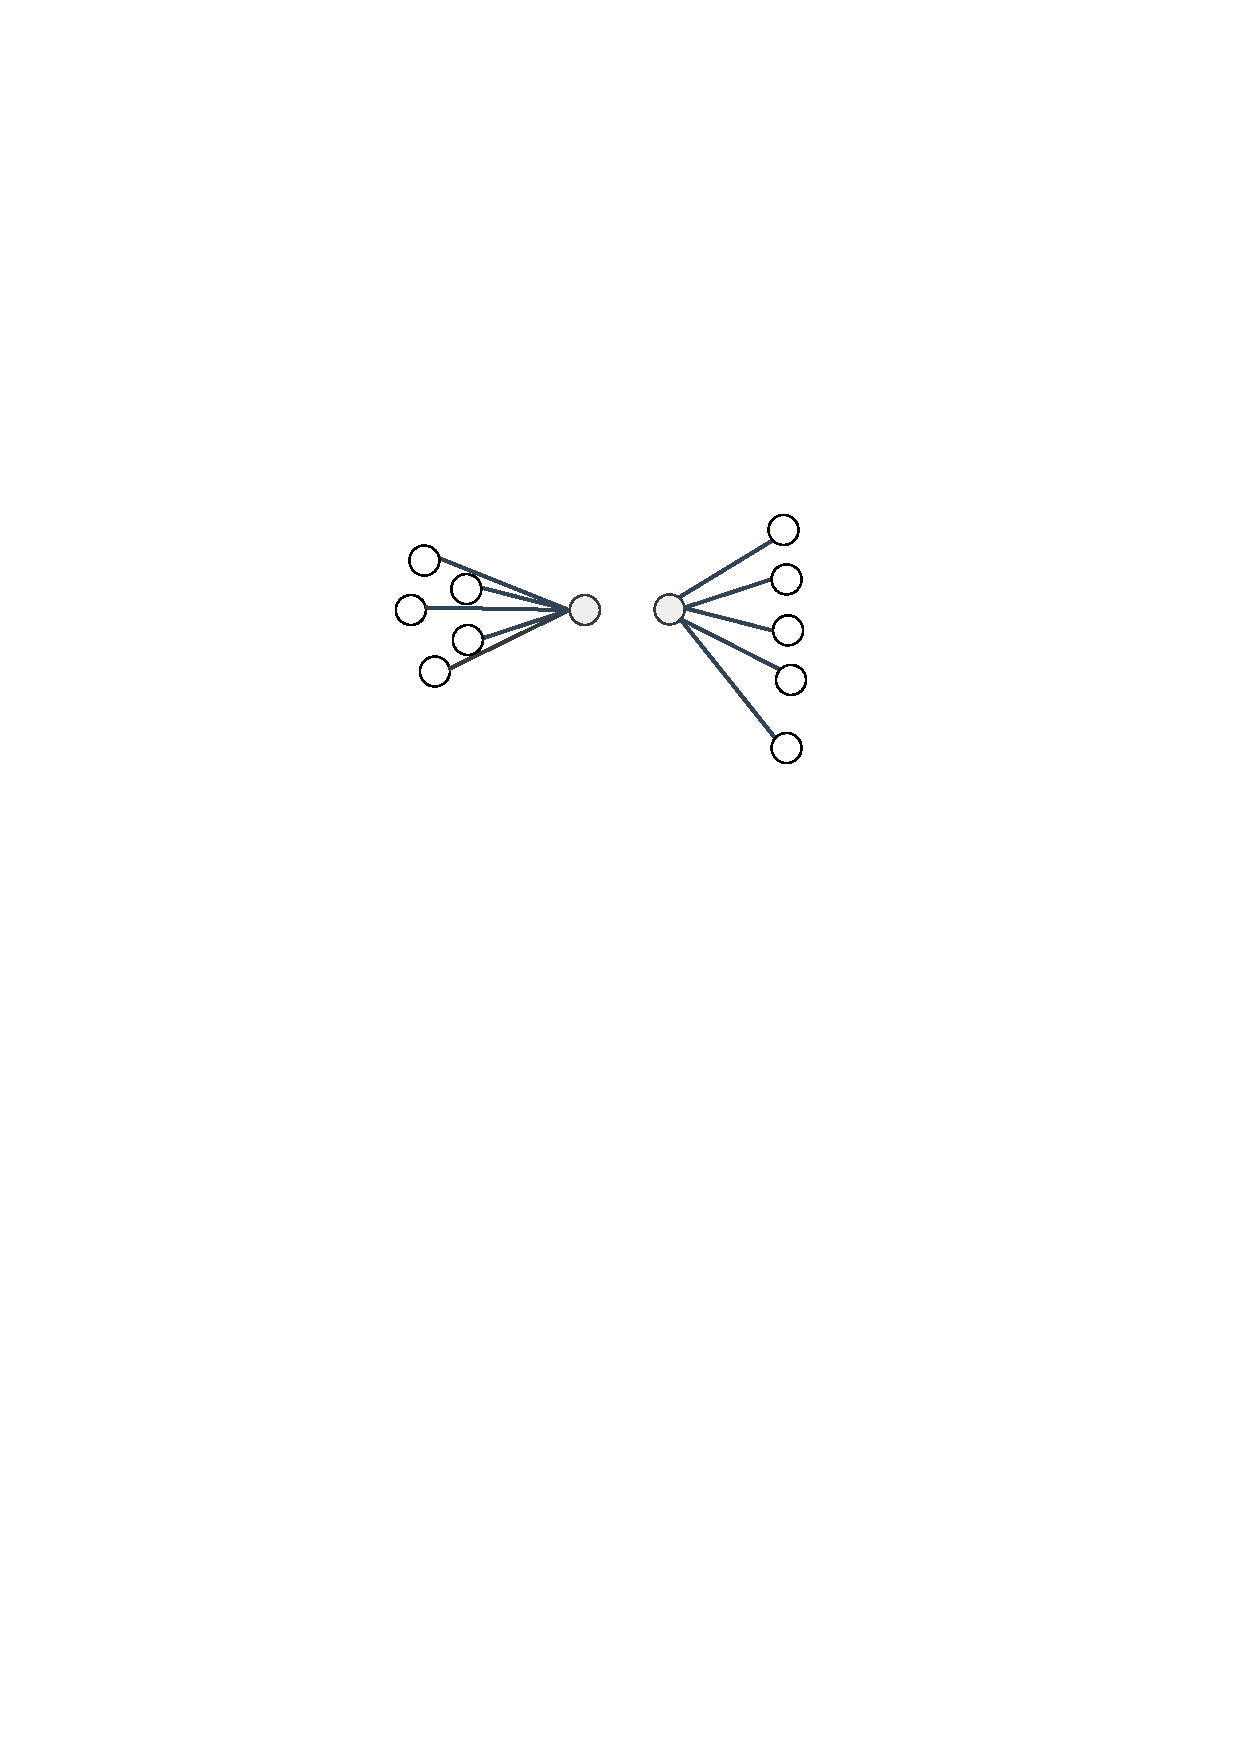
\includegraphics[scale=.6]{figures/followers/follower1}
        \caption{2 seeds with an equal number of followers...}
        \label{fig:follower1}
    \end{subtable}
     \begin{subtable}{1\textwidth}
        \centering
        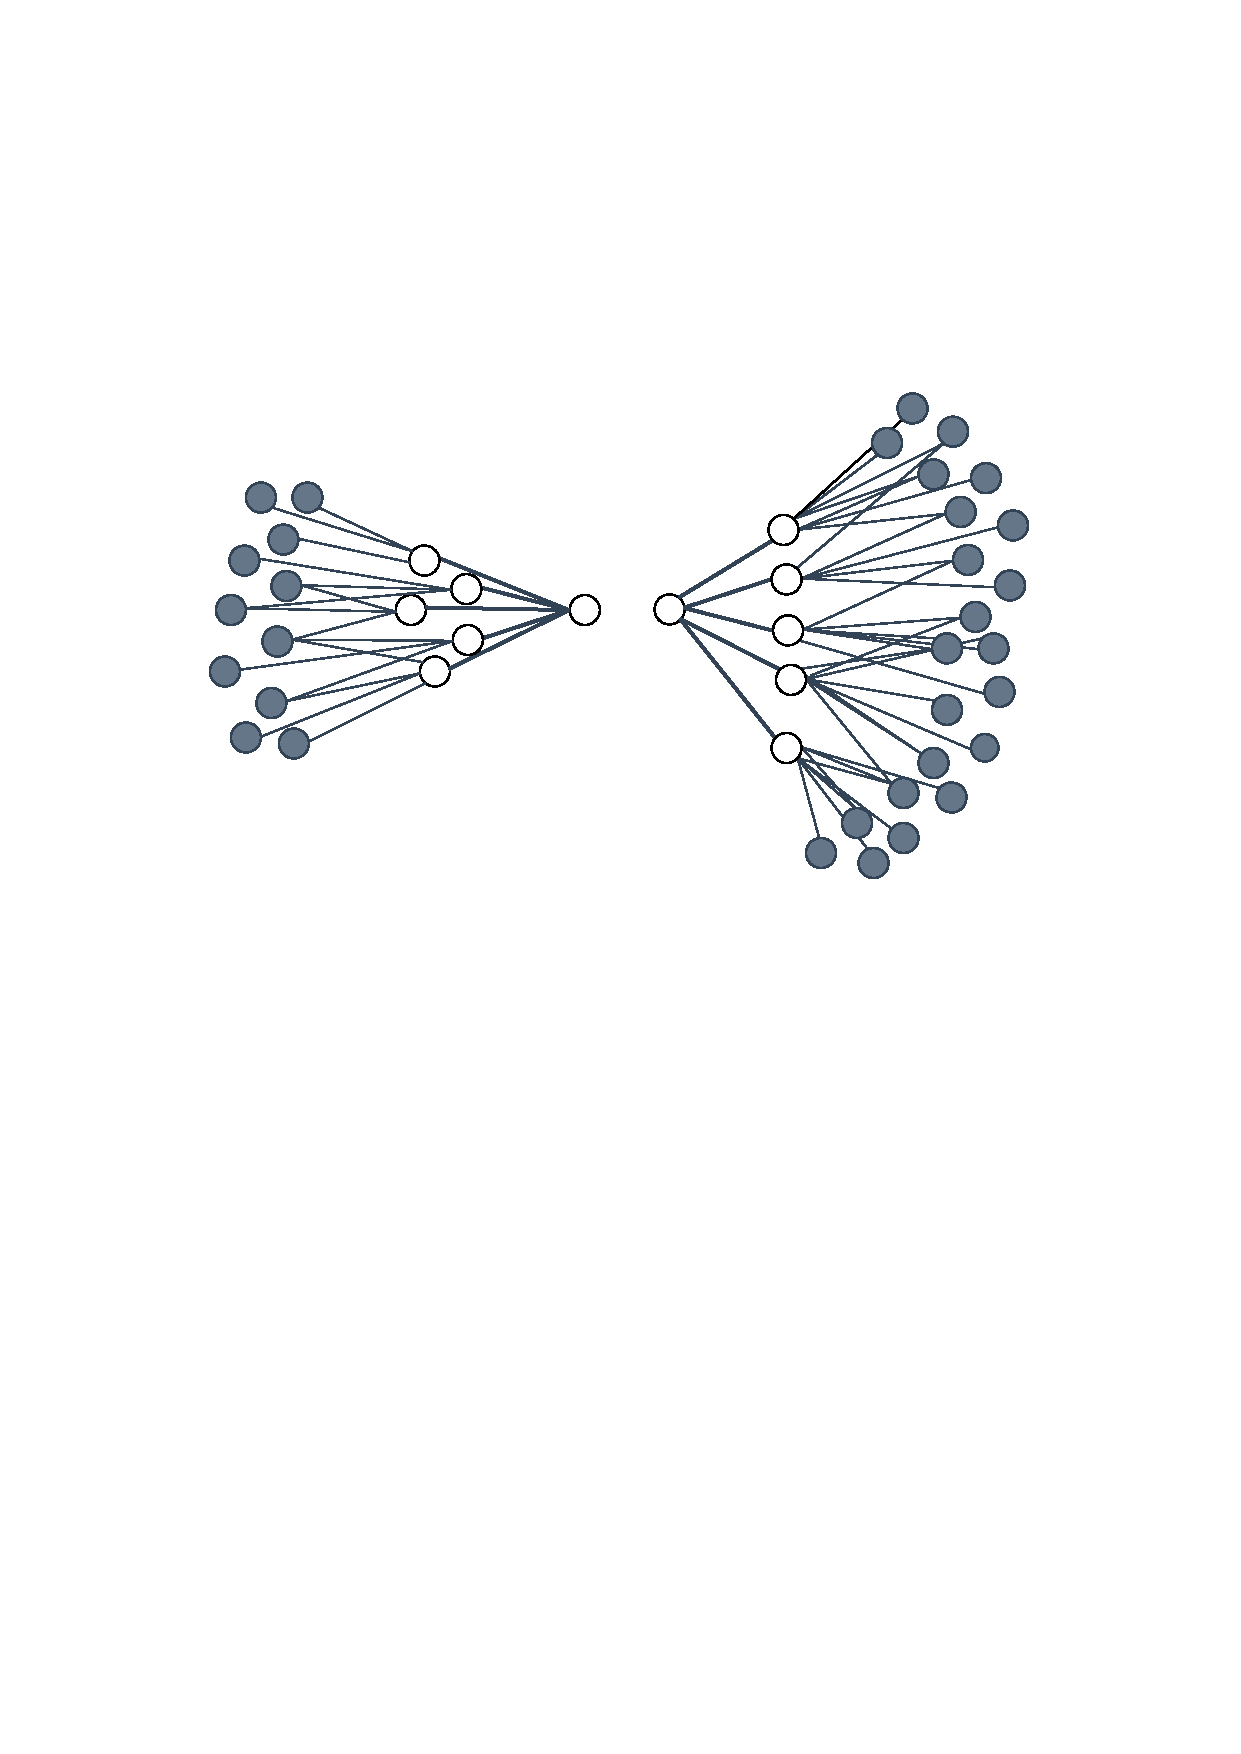
\includegraphics[scale=.6]{figures/followers/follower2}
        \caption{... but different numbers of followers}
        \label{fig:follower2}
    \end{subtable}
    \begin{subtable}{1\textwidth}
     \centering
        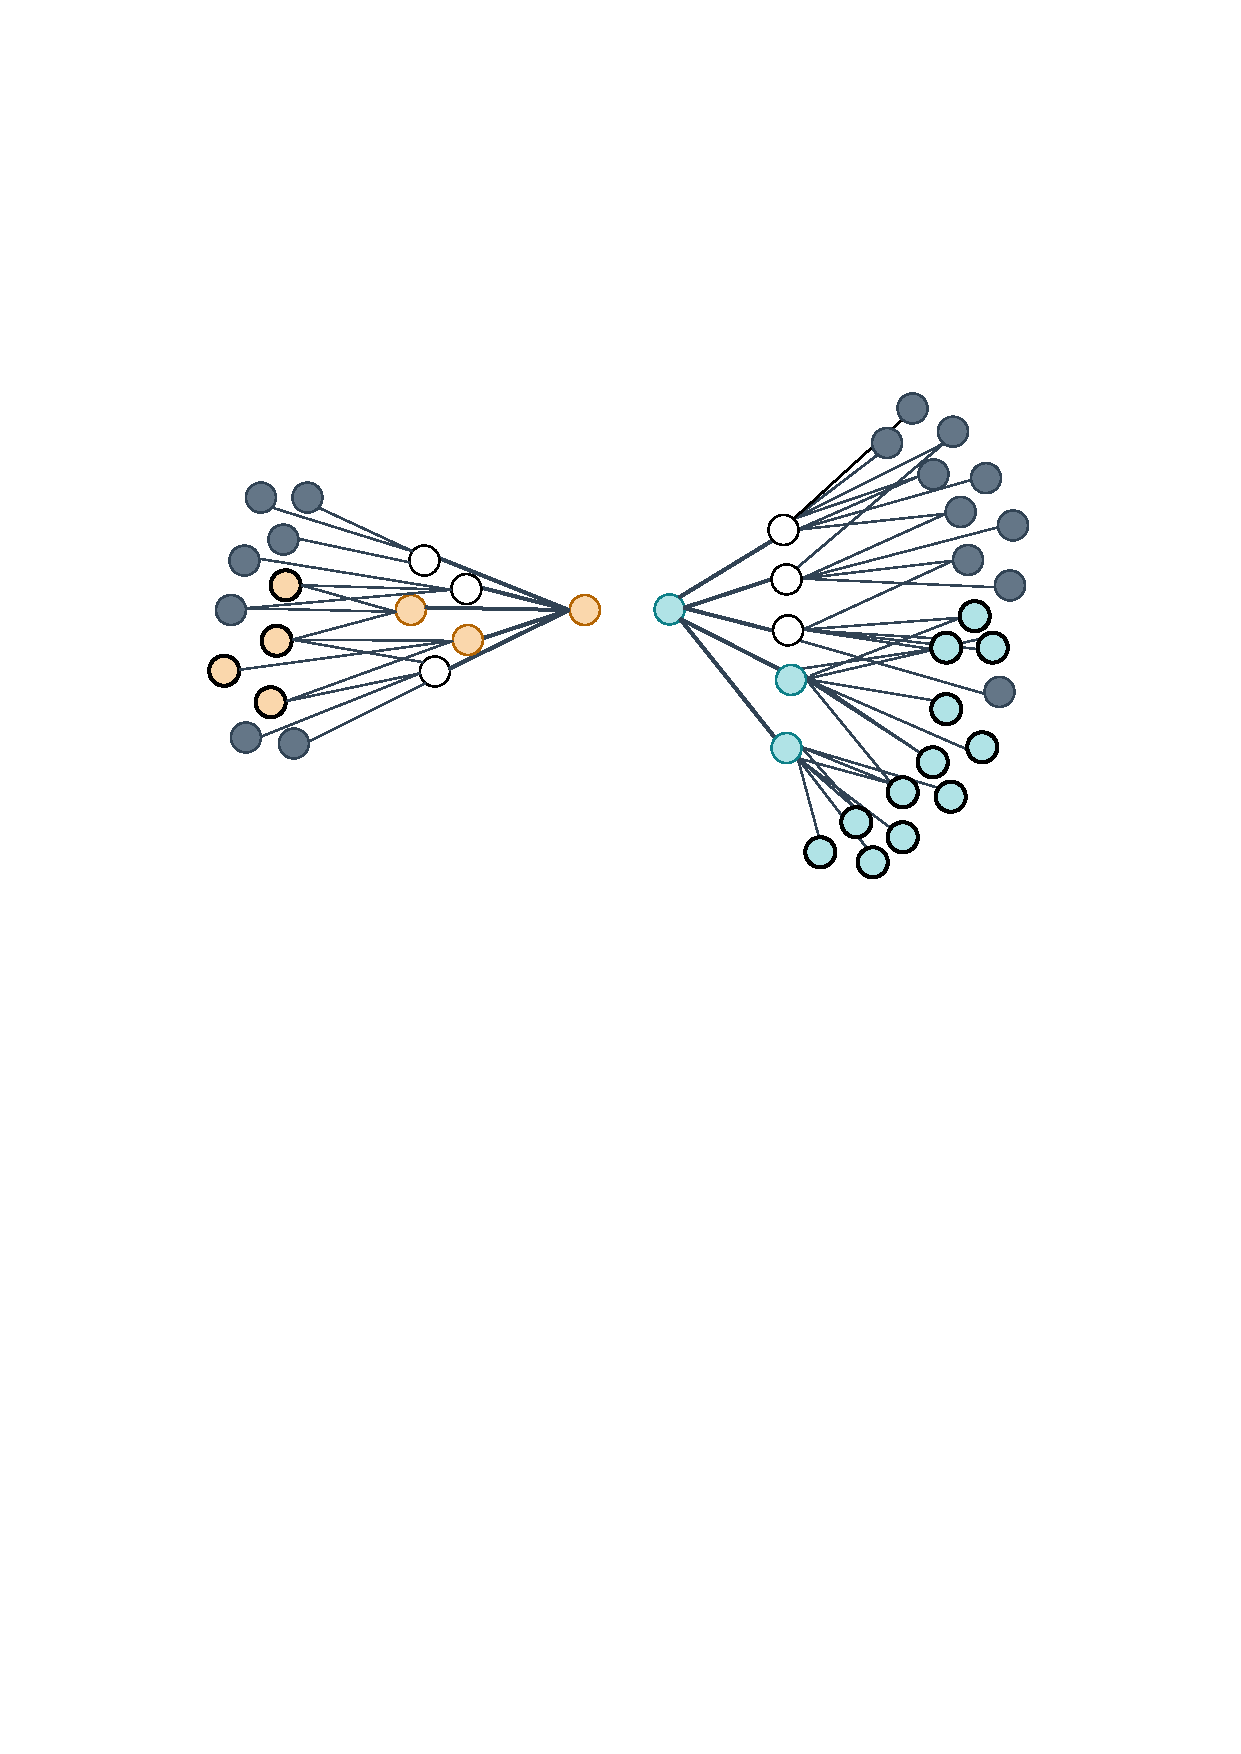
\includegraphics[scale=.6]{figures/followers/follower3}
        \caption{, leading to different numbers of tweet impressions}
        \label{fig:follower3}
    \end{subtable}
\end{center}
\begin{spacing}{0.5}
		{\footnotesize \textbf{Notes:} The Figure illustrates the IV strategy we develop in this article, in the spirit of an intention-to-treat approach. The thought experiment is described in detail in the text.}
\end{spacing}
\vspace{.5cm}	
\caption{IV strategy: Illustration}
\label{fig:follower}
\end{figure}
% 	\subfloat[][\textbf{... but different number of followers' followers}]{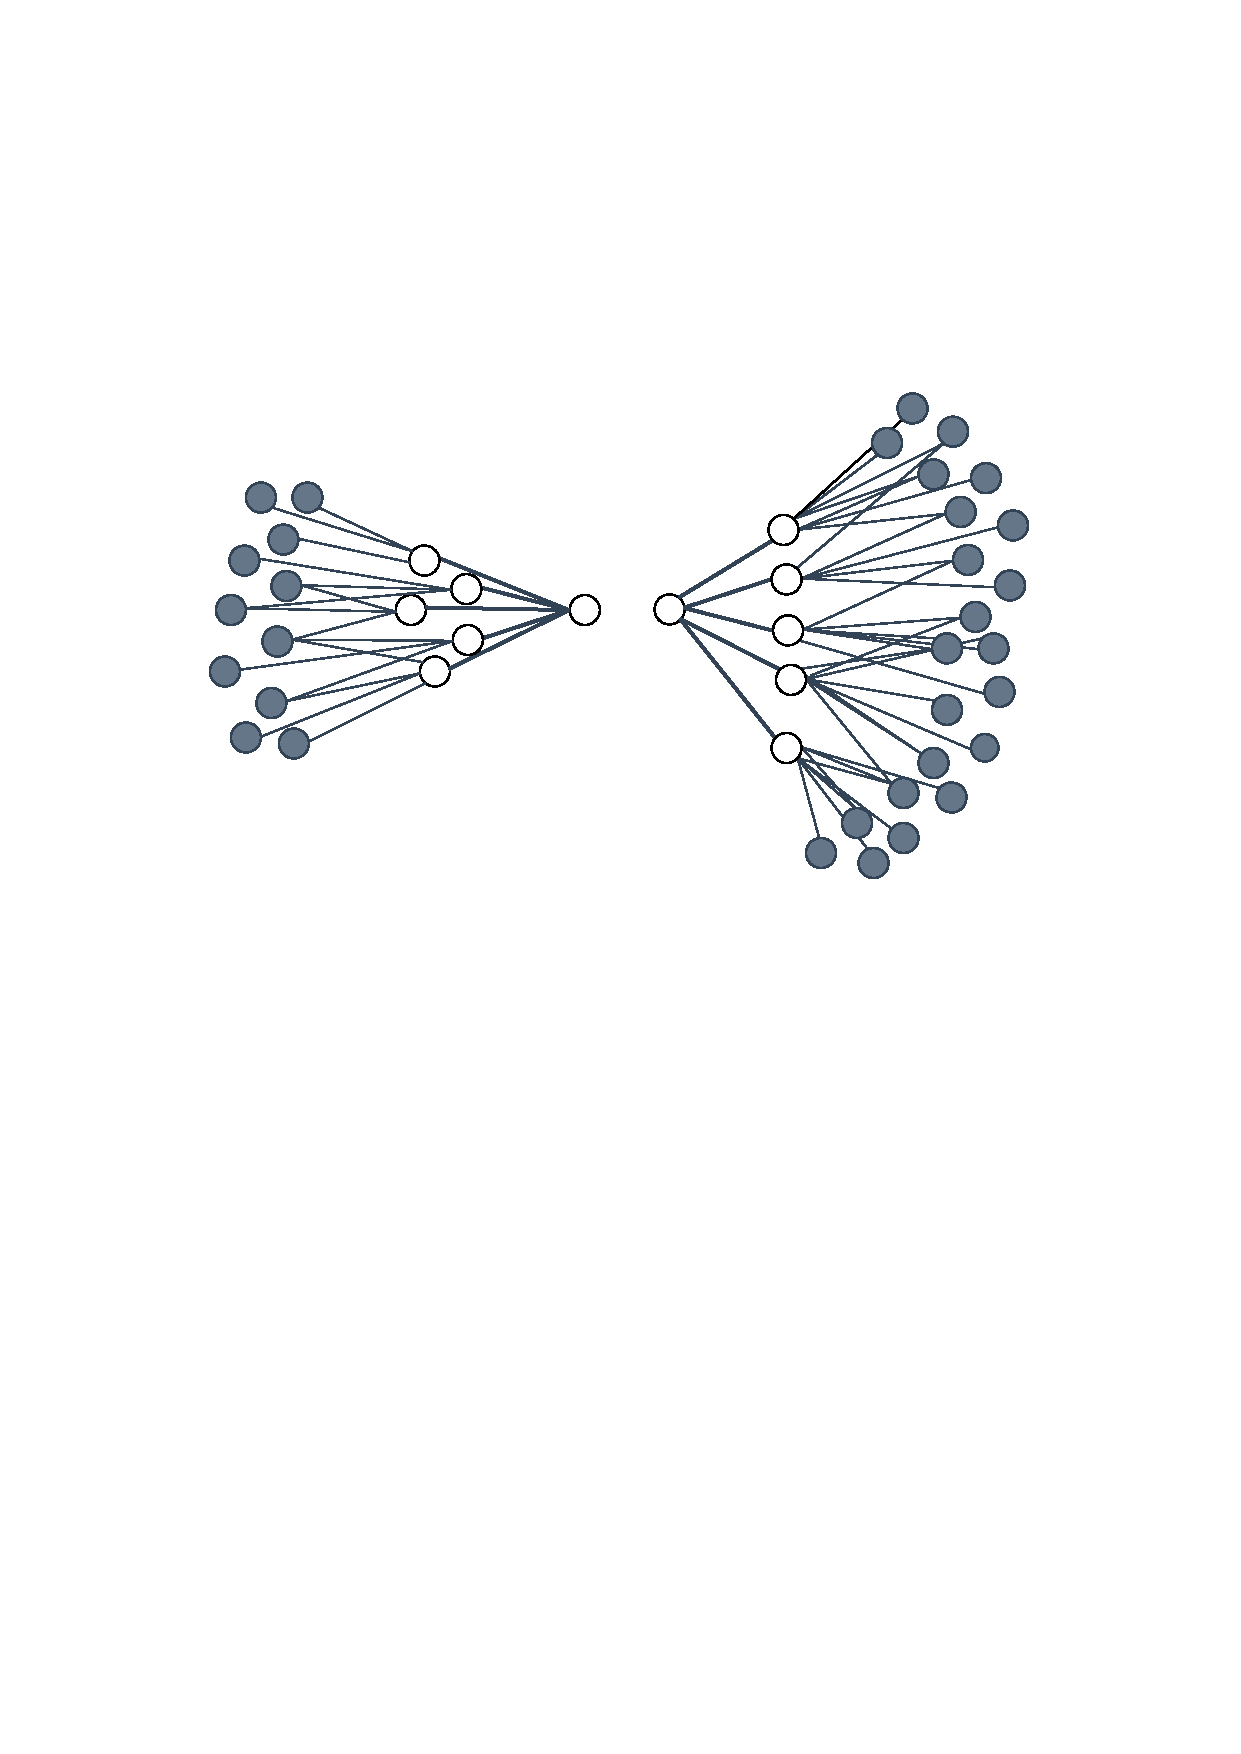
\includegraphics[scale=.6]{figures/followers/follower2}
% \label{fig:follower2}}
% \quad
% 	\subfloat[][\textbf{, leading to different number of tweets' impressions}]{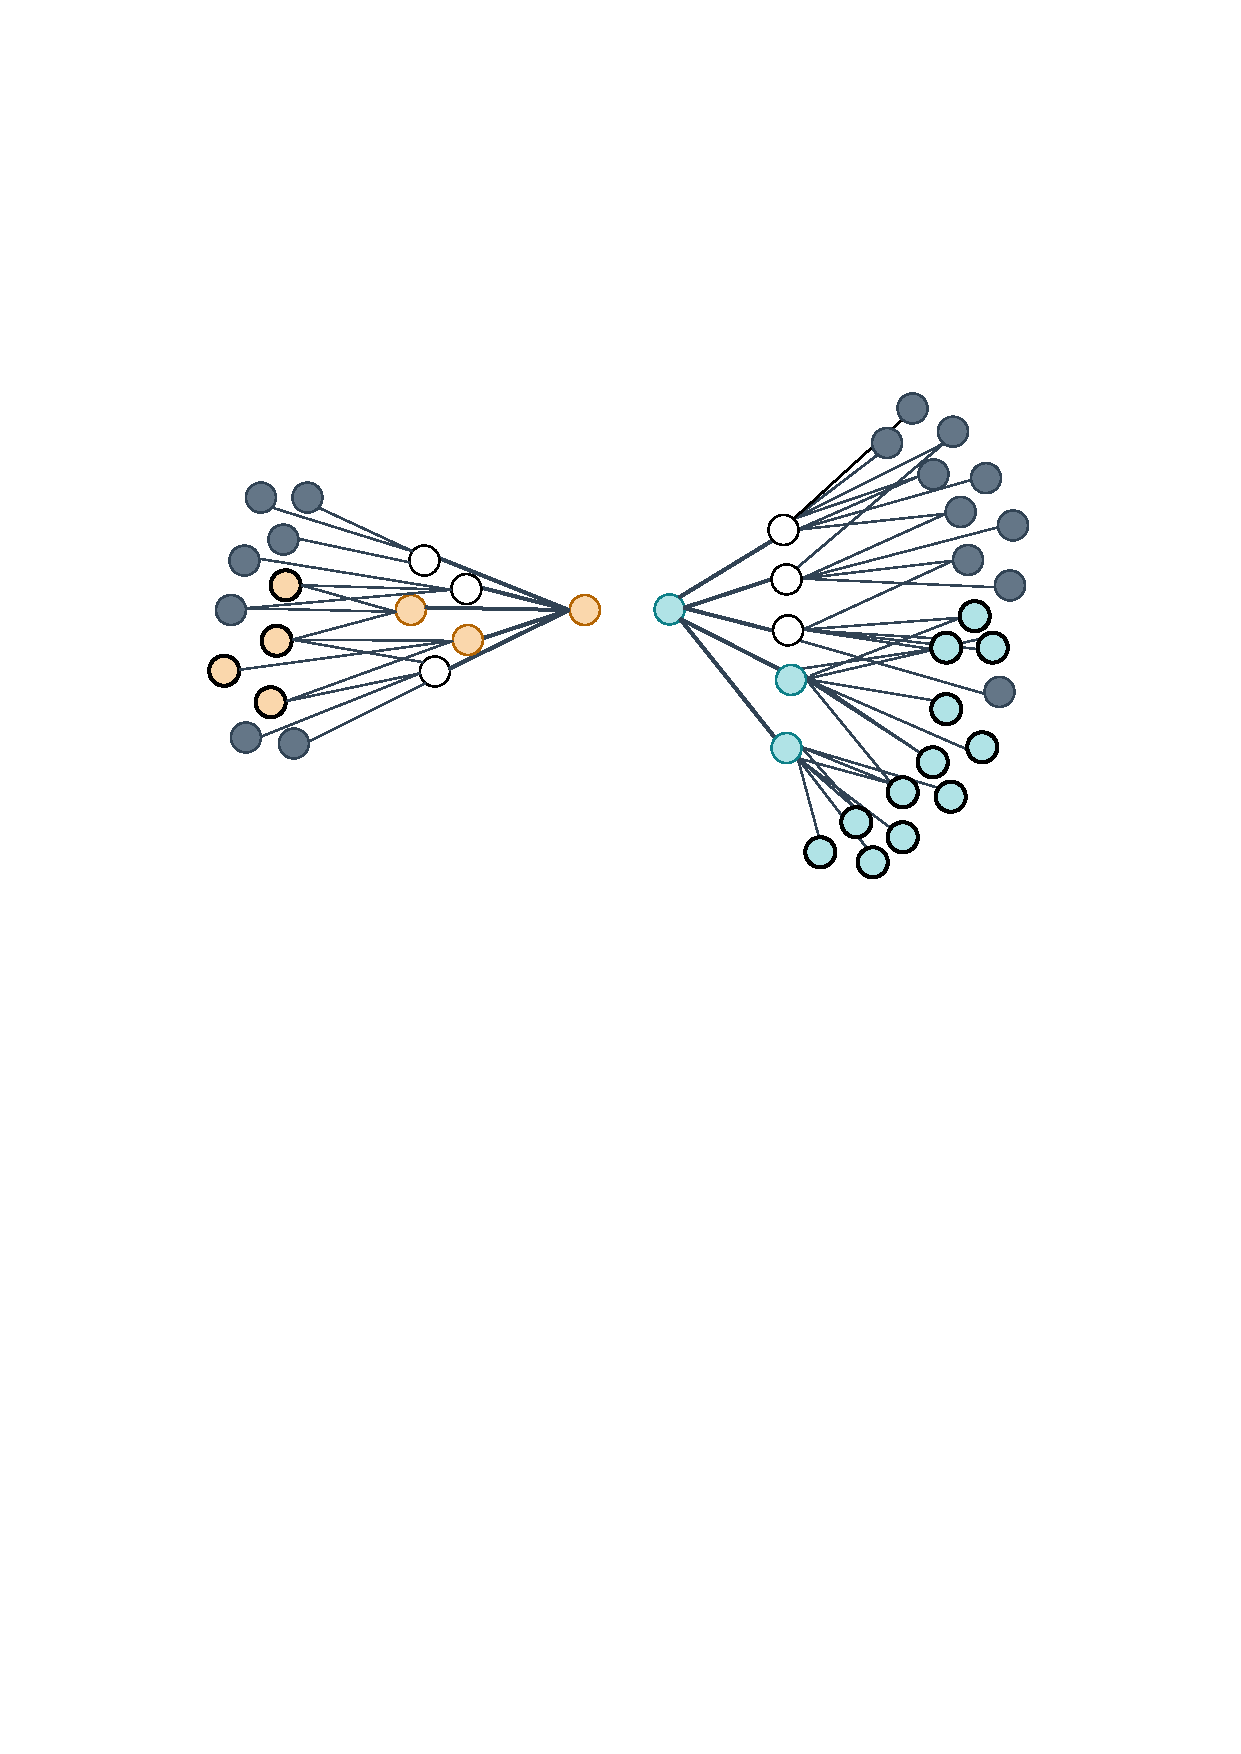
\includegraphics[scale=.6]{figures/followers/follower3}
% \label{fig:follower3}}
% \end{center}
% 	\begin{spacing}{0.5}
% 		{\footnotesize \textbf{Notes:} The Figure illustrates the IV strategy we develop in this article, in the spirit of an intention-to-treat approach. The thought experiment is described in details in the text.}
% 	\end{spacing}
% \vspace{.5cm}	

% %%%%%%%%%%%%%%%%%%%%%%%%%%%%%%%%%%%%%%%%%%%%%%%%%%%%%%%%%%%%%%%%%%%%%% 


However, while presumably more exogenous than the previous approach, the number of impressions generated by the seeds' followers may still suffer from the fact that a seed's centrality in the Twitter network may be related to its ability to produce newsworthy content. To relax the exclusion restriction, the instrument we propose is the interaction between the seed's centrality in the network (as previously defined) and the news pressure at the time of the tweet (measured by the number of interactions generated by all the tweets published in the hour preceding the tweet), controlling for the direct effect of centrality and news pressure.\footnote{We thank Katia Zhuravskaya for suggesting this approach.} Our identification assumption is that, once we control for the direct effects of centrality and news pressure, the interaction between the seed's centrality and news pressure should only affect traditional news production through its effect on the tweet's visibility on Twitter.
% (if you control for the direct effect of the centrality, which could be correlated with the quality of the content, and for the news pressure, which could affect both the twitter users' and the media's attention at the same time.)


We show that, at the event-level, an increase of $1,000$ in the number of tweets published before the first media article appears is associated with an increase of $2$ in the number of media articles published in the event; this increase is partly driven by a higher number of media outlets covering the event. Importantly, these results are robust to controlling for the endogeneity of the event popularity on Twitter, and to the use of a number of different empirical specifications.

We then turn to the media-level analysis and investigate the heterogeneity of our results on the characteristics of the media outlets. For each of the media outlets in our sample, we collect information on their social media presence, as well as on their business model (e.g. whether they put part of their content behind a paywall and their reliance on advertising revenues). In addition, for a subset of the media, we also gather information on the size of their newsroom, which provides us with a proxy on their investment in news quality. Ultimately, we also investigate whether there is heterogeneity depending on the offline format of the media. We show that the magnitude of the effect is stronger for the media whose social media presence is relatively higher.
%  depending on the topic of the event (e.g. sport, international affairs, economics, etc.), as well as 
% We find that \textbf{A COMPLETER} 

Finally, we discuss the mechanisms that may help rationalizing our findings. First, journalists monitor Twitter. For example, the Muck Rack’s  ``State of Journalism 2019" report reveals that nearly $60\%$ of reporters turn to digital newspapers or magazines as their first source of news, and $22\%$ check Twitter first. This may help us to understand why a number of stories emerge first on Twitter and the high reactivity of mainstream media, but it does not explain why the intensity of the media coverage (on the intensive margin) varies with the popularity of a story on Twitter. In the absence of perfect information about consumer preferences, publishers may use Twitter as a signal that allows them to draw inferences about what news consumers are interested in. Finally, social media and mainstream media compete for readers' attention. This may affect mainstream media incentives to invest in quality.

\medskip
The rest of this chapter is composed as follows: first, we detail our contributions to the literature in the Section below.  We then describe our data and specify how we measure popularity on Twitter and media coverage. In Section \ref{Sec:EmpiricalSpecification}, we present our empirical specification, and in particular the new instrument we propose to identify the causal impact of a story's popularity on the subsequent news coverage it receives. We then present our results and analyze various dimensions of heterogeneity in Section \ref{Sec: results}. Finally, we discuss the mechanisms at play in Section \ref{Sec:Mechanisms}.

%%%%%%%%%%%%%%%%%%%%%%%%%%%%%%%%
\section{Literature review}

We contribute to the growing literature on the impact of the introduction of new media technologies on political participation, government accountability and electoral outcomes (see among others \citet{Gentzkowetal2011,SnyderStromberg2010} on newspapers; \citet{Stromberg2004} on radio; \citet{Gentzkow2006,AngelucciCage2019,AngelucciCageSinkinson2020} on television, and \citet{BoxellGentzkowShapiro2018,Gavazzaetal2019} on the Internet). There are very few papers examining how social media affects voting \citep[for a review of the literature see][]{Zhuravskayaetal2020}, and these mainly concentrate on the role played by fake news \citep{AllcottGentzkow2017}. So far, the focus of this literature has mostly been on news consumption, and little is known about the empirical impact social media have on news production by mainstream media. One exception is a work-in-progress article by \citet{HatteMadinierZhuravskaya2020}  who study the effect of Twitter on the US  TV coverage of the Israeli-Palestinian conflict. Compared to this work, our contribution is threefold. First, we focus on the overall activity on Twitter and collect a large representative sample of about 70\% of all tweets (about $1.8$ billion tweets) rather than the tweets associated with a small number of keywords. Second, we develop an instrument for measuring popularity shocks on Twitter based on the structure of the network that could be of use in different contexts rather than relying on an Internet outage instrument (which affects all electronic communications, access to online media, etc., and not only access to Twitter). Finally, we investigate whether there are heterogeneous effects depending on the media characteristics, in particular their business model and their reliance on advertising revenues.

An expanding theoretical literature studies the effects of social media on news. \Citet{deCorniereSarvary2019} develop a model where consumers allocate their attention between a newspaper and a social platform \citep[see also][for a theory of news coverage in environments of information abundance]{AlaouiGermano2020}. They document a negative impact on the media's incentives to invest in quality. This literature mainly concentrates on competition for attention between newspapers and social media, and documents a trade-off between the business-stealing and the readership-expansion effect of platforms \citep{JeonNasr2016}.\footnote{See \citet{Jeon2018} for a survey of articles on news aggregators.}  Here, we highlight the fact that not only are mainstream and social media competing for attention, but also that social media can be used by mainstream media as a source of news as well as a signal to draw inferences on consumers' preferences. We investigate empirically how a story's popularity on Twitter impacts the information produced by traditional media, and in particular the intensity of the coverage they devote to that story.

Our results also contribute to the growing literature in the fields of Economics and Political Science using social media data, and in particular the structure of the social networks -- usually Twitter -- as a source of information on the ideological positions of actors \citep{Barbera2015,cardon2019unfolding}, the importance of ideological segregation and the extent of political polarization \citep{HalberstamKnight2016,Giavazzietal2020}, and political language dissemination \citep{Longhietal2019}.\footnote{See also \citet{Barberaetal2019} who use Twitter data to analyze the extent to which politicians allocate attention to different issues before or after shifts in issue attention by the public.} \citet{Gorodnichenkoetal2018} study information diffusion on Twitter, and \citet{AllcottGentzkowYu2019_ReasearchPolitics} the spread of false content. While this literature mostly focuses on relatively small corpuses of tweets and on corpuses that are not representative of the overall activity on Twitter \citep[e.g.][make requests to collect tweets using Brexit-related keywords]{Gorodnichenkoetal2018}, we build a representative corpus of tweets and impose no restriction on the data collection. Furthermore, we contribute to this literature by considering the propagation of information on social media as well as by studying whether and how information propagates from social media to mainstream media (and vice versa). While \citet{CageHerveViaud2020} only consider news propagation on mainstream media, we investigate here the extent to which the popularity of a story on social media affects the coverage devoted to this story by traditional media outlets.

The impact of ``popularity" on editorial decisions has been studied by \citet{SenYildirim2015} who use data from an Indian English daily newspaper to investigate whether editors expand online coverage of stories which receive more clicks initially.\footnote{See also \citet{ClaussenPeukertSen2019} who use data from a German newspaper to investigate whether automated personalized recommendation outperforms human curation in terms of user engagement.} Compared to this previous work, our contribution is threefold. First, we use the entire universe of French general information media online (around $200$ media outlets), rather than one single newspaper. Second, we not only identify the role played by popularity, but also investigate whether there is heterogeneity depending on the characteristics of the media outlets, as well as the topic of the story. Third, we consider both the extensive and the intensive  margin\footnote{The intensive margin here corresponds to whether a story is covered, while on the extensive margin we consider both the total number of articles (conditional on covering the story) and the characteristics of these articles.}, rather than focusing on the subset of stories that receive at least some coverage in the media. Finally, we also contribute to the empirical literature on media by using a split-sample approach; while this approach is increasingly used in economics with the pre-registration of Randomized Controlled Trials, we believe we are the very first to use it with ``real-world data" on such a large scale.

In addition to this, we contribute to the broader literature on social media that documents its impact on racism \citep{MullerSchwarz2019}, political protests \citep{EnikolopovMakarinPetrova2020}, the fight against corruption \citep{Enikolopovetal2018}, and the size of campaign donations \citep{Petrovaetal2017}. Overall, social media is a technology that has both positive and negative effects \citep{Allcottetal2020}. This also holds true for its impact on traditional media: we contribute to this literature by documenting the complex effects social media has on news production, and consequently on news consumption.

Finally, our instrumentation strategy is related on the one hand to the literature that looks at the quantity of newsworthy material at a given moment of time \citep[e.g.][]{EisenseeStromberg2007,DjourelovaDurante2019}, and on the other hand to the literature on network interactions \citep[see][for a recent survey]{BramoulleDjebbariFortin2020}. The main issue faced by researchers willing to identify the causal effects of peers is that the structure of the network itself may be endogenous. Here, we relax the concern of network endogeneity by considering the interaction between the network and news pressure at a given moment of time.





%%%%%%%%%%%%%%%%%%%%%%%%%%%%%%%%%%%%%%%%%%%%%%%%%%%%%%%%%%%%%%%%
%%%%%%%%%%%%%%%%%%%%%%%%%%%%%%%%%%%%%%%%%%%%%%%%%%%%%%%%%%%%%%%%
\section{Data and descriptive statistics\label{Sec:DataAlgorithms}}
%%%%%%%%%%%%%%%%%%%%%%%%%%%%%%%%%%%%%%%%%%%%%%%%%%%%%%%%%%%%%%%%
%%%%%%%%%%%%%%%%%%%%%%%%%%%%%%%%%%%%%%%%%%%%%%%%%%%%%%%%%%%%%%%%

The new dataset we built for this study is composed of two main data sources that we have collected and merged: on the one hand, a representative sample of tweets, and on the other hand, the online content of the general information media outlets. In this section, we describe these two datasets in turn.


%%%%%%%%%%%%%%%%%%%%%%%%%%%%%%%%%
\subsection{Data: Tweets\label{Sec:DataTweets}}
%%%%%%%%%%%%%%%%%%%%%%%%%%%%%%%%%

First, we collect a representative sample of all the tweets in French during an entire year: July 2018-July 2019. Our dataset, which contains around $1.8$ billion tweets, encompasses around $70\%$ of all tweets in French (including retweets) during this time period (see Chapter \ref{Chapter: Corpus} Section \ref{Evaluate the share} for a discussion of the completeness of our dataset). For each of these tweets, we collect information on their ``success" on Twitter (number of likes or comments, etc.), as well as information on the user's characteristics at the time of the tweet (e.g. number of followers).

%%%%%%%%%%%%%%%%%%%%%%%%%%%%%%%%%
\subsubsection{Filtering the tweets}

An important issue on Twitter is the use of bots, i.e. non-human actors and trolls publishing tweets on the social media  \citep[see e.g.][]{Gorodnichenkoetal2018}. In recent years, Twitter has been actively cracking down on bots. In our analysis, we do perform some filtering designed to limit the share of tweets from bots in our dataset. However we do not remove all automated accounts: many media accounts, for example, post some content automatically, and are not considered to be bots. Moreover, some types of automatic behaviors on Twitter, such as automatic retweets, may contribute to the popularity of stories and therefore should be kept in our dataset.

Our filtering rules are as follows. First, we use the ``source" label provided by Twitter for each tweet.\footnote{Twitter describes this label as follows: ``Tweet source labels help you better understand how a Tweet was posted. This additional information provides context about the Tweet and its author. If you don’t recognize the source, you may want to learn more to determine how much you trust the content. [...] Authors sometimes use third-party client applications to manage their Tweets, manage marketing campaigns, measure advertising performance, provide customer support, and to target certain groups of people to advertise to. Third-party clients are software tools used by authors and therefore are not affiliated with, nor do they reflect the views of, the Tweet content. Tweets and campaigns can be directly created by humans or, in some circumstances, automated by an application."} 
Tweets emanating from a ``source" such as ``Twitter for iPhone" can be considered valid; however, we excluded sources explicitly described as bots, or referring to gaming or pornographic websites. We also excluded apps automatically posting tweets based on the behaviour of users: for example, many Twitter users (who are human beings and usually publish tweets they have written themselves) post automatic tweets such as ``I like a video on Youtube: [url]". The entire list of the excluded sources is presented in Table \ref{tab:botlist} of the \hyperlink{ref:Appendix}{Appendix}. 

Second, we filter the users depending on their activity on the network: we only keep users with fewer than 1,000 tweets a day\footnote{As a matter of comparison, the Twitter account of \textit{Le Monde} publishes on average 88 tweets per day, and that of \textit{Le Figaro} 216.}, and the users who have at least 1 follower. Finally, we only keep the users who have at least 3 tweets in French between July and September 2018.


%%%%%%%%%%%%%%%%%%%%%%%%%%%%%%%%%
\subsubsection{Descriptive statistics}

%Table \ref{Tab:sum_stat_tweets_201809_201902} provides summary statistics on the tweets we collected. For each of the tweets, we have information on its length ($101$ characters on average or $6.1$ words), and know whether it is a retweet of an existing tweet or an original tweet. $63\%$ of the tweets in our dataset are retweets; some of these retweets are ``quotes", i.e. comment on the retweeted tweet.\footnote{Quote Tweets share another tweet with an additional comment, unlike Retweets that repost the original tweet without any modification.} Of the original tweets, some are in reply to other tweets ($18\%$ of the tweets in our sample). Finally, $12\%$ of the tweets contains a URL, most often a link to a news media article or a video.
%
%We also gather information on the popularity of each of the tweets in our sample. On average, the tweets are only retweeted $0.8$ times, liked $1.5$ times, and receive $0.1$ replies (these numbers are only computed on the original tweets, given that retweets, likes and quotes are not attributed to the Retweets but to the original tweets).
%
%
%%%%%%%%%%%%%%%%%%%%%%%%%%%%%%%%%%%%%%%%%%%%%%%%%%%%%%%%%%%%%%%%%%%%%%%
%\begin{sidewaystable}
%\caption{Summary statistics: Tweets (full sample) \textbf{COMPLETER AVEC LA VERSION A JOUR -- ET RAJOUTER EGALEMENT STAT DES SUR FULL SAMPLE OF USERS}}
%\begin{center}
%	{
\def\sym#1{\ifmmode^{#1}\else\(^{#1}\)\fi}
\begin{tabular}{l*{1}{ccccccc}}
\hline\hline
                    &\multicolumn{7}{c}{}                                                                      \\
                    &        Mean&      St.Dev&         P25&      Median&         P75&         Max&         Obs\\
\hline
\textbf{Characteristics of the tweet}&            &            &            &            &            &            &            \\
Length of the tweet (nb of characters)&         101&          54&          59&          97&         140&       1,415&1,030,423,899\\
Number of words     &         6.1&         4.1&         3.0&         6.0&         8.0&       269.0&1,030,423,899\\
=1 if tweet contains an URL&        0.12&        0.33&        0.00&        0.00&        0.00&        1.00&1,030,423,899\\
=1 if the tweet is a retweet&        0.63&        0.48&        0.00&        1.00&        1.00&        1.00&1,030,423,899\\
=1 if the tweet is a reply&        0.18&        0.39&        0.00&        0.00&        0.00&        1.00&1,030,423,899\\
=1 if the tweet is a quote&        0.20&        0.40&        0.00&        0.00&        0.00&        1.00&1,030,423,899\\
\textbf{Popularity of the tweet}&            &            &            &            &            &            &            \\
Number of retweets  &         0.8&        65.8&         0.0&         0.0&         0.0&   365,931.0&1,030,423,897\\
Number of replies   &         0.1&         5.0&         0.0&         0.0&         0.0&    49,218.0&1,030,423,897\\
Number of likes     &         1.5&       115.8&         0.0&         0.0&         0.0&   980,681.0&1,030,423,899\\
\textbf{Characteristics of the user}&            &            &            &            &            &            &            \\
Total nb of Tweets  &      35,798&     300,554&       2,312&       9,902&      32,403&  20,389,037&1,030,423,899\\
Nb of followers     &       3,225&      73,841&          96&         279&         742& 106,815,712&1,030,423,899\\
Nb of users the account is following&         669&       3,946&         124&         258&         559&   1,829,616&1,030,423,899\\
=1 if user is a media&       0.001&       0.036&       0.000&       0.000&       0.000&       1.000&1,030,423,899\\
=1 if user is a journalist&       0.002&       0.043&       0.000&       0.000&       0.000&       1.000&1,030,423,899\\
\hline\hline
\end{tabular}
}

%\end{center}
%\begin{spacing}{0.5}
%	{\fns \textbf{Notes:} The table gives summary statistics. Time period is July 2018-July 2019. Variables are values for all the tweets included in our dataset. Variables are described in more details in the text.} 
%\end{spacing}
%\label{Tab:sum_stat_tweets_201809_201902}
%\end{sidewaystable} 
%%%%%%%%%%%%%%%%%%%%%%%%%%%%%%%%%%%%%%%%%%%%%%%%%%%%%%%%%%%%%%%%%%%%%%%
%

%%%%%%%%%%%%%%%%%%%%%%%%%%%%%%%%%

As highlighted in the introduction, to address concerns about specification search and publication bias \citep{Leamer1978,Leamer1983,Glaeser2006_incentives}, we implement a split-sample approach in this paper \citep{FafchampsLabonne2016,FafchampsLabonne2017,AndersonMagruder2017}. We split the data into two non-overlapping datasets: July 2018-September 2018 and October 2018-July 2019. In this chapter, we use the three-month dataset covering July 2018-September 2018 to narrow down the list of hypotheses we wish to test.

The final paper will only use data from October 2018 to July 2019. The idea here is to avoid multiple hypothesis testing, which has been shown to be an issue in experimental economics \citep{ListShaikhXu2019} and could also be of concern here. Hence, for the remainder of the chapter, we will rely solely on the first three months of our dataset. This sample includes $417,153,648$ tweets; Table \ref{Tab:sum_stat_tweets_split_sample} presents summary statistics for these tweets. 

For each of the tweets, we have information on its length ($102$ characters on average or $6.2$ words), and know whether it is a retweet of an existing tweet or an original tweet. $63\%$ of the tweets in our dataset are retweets; some of these retweets are ``quotes", i.e. comment on the retweeted tweet.\footnote{Quote tweets are much like retweets except that they include a new tweet message.} Of the original tweets, some are replies to other tweets ($17\%$ of the tweets in our sample). Finally, $13\%$ of the tweets contains a URL, most often a link to a news media article or to a video.

We also gather information on the popularity of each of the tweets in our sample. On average, the tweets are retweeted $2.3$ times, liked $3.7$ times, and receive $0.2$ replies (these numbers are only computed on the original tweets, given that retweets, likes and quotes are not attributed to the retweets but to the original tweets).\footnote{\hyperlink{ref:Appendix}{Appendix} Table \ref{Tab:sum_stat_tweets_split_sample_bflitre} shows statistics on the sample of tweets we collect before applying the filters to exclude the bots as described above.} 


%%%%%%%%%%%%%%%%%%%%%%%%%%%%%%%%%%%%%%%%%%%%%%%%%%%%%%%%%%%%%%%%%%%%%%
\begin{sidewaystable}
\caption{Summary statistics: Tweets (split-sample, July 2018-September 2018)}
\begin{center}
	{
\def\sym#1{\ifmmode^{#1}\else\(^{#1}\)\fi}
\begin{tabular}{l*{1}{ccccccc}}
\hline\hline
                    &\multicolumn{7}{c}{}                                                                      \\
                    &        Mean&      St.Dev&         P25&      Median&         P75&         Max&         Obs\\
\hline
\textbf{Characteristics of the tweet}&            &            &            &            &            &            &            \\
Length of the tweet (nb of characters)&         102&          52&          61&          98&         140&       1,121& 417,153,648\\
Number of words     &         6.2&         4.0&         3.0&         6.0&         9.0&         269& 417,153,648\\
=1 if tweet contains an URL&        0.13&        0.33&        0.00&        0.00&        0.00&           1& 417,153,648\\
=1 if the tweet is a retweet&        0.63&        0.48&        0.00&        1.00&        1.00&           1& 417,153,648\\
=1 if the tweet is a reply&        0.17&        0.38&        0.00&        0.00&        0.00&           1& 417,153,648\\
=1 if the tweet is a quote&        0.19&        0.39&        0.00&        0.00&        0.00&           1& 417,153,648\\
\textbf{Popularity of the tweet}&            &            &            &            &            &            &            \\
Number of retweets  &         2.3&       111.5&       0.000&       0.000&       0.000&     117,389& 154,273,618\\
Number of replies   &         0.2&         6.6&       0.000&       0.000&       0.000&      47,892& 154,273,618\\
Number of likes     &         3.7&       172.2&       0.000&       0.000&       0.000&     449,881& 154,273,619\\
\hline\hline
\end{tabular}
}

\end{center}
\begin{spacing}{0.5}
	{\fns \textbf{Notes:} The table gives summary statistics. Time period is July 2018-September 2018. Variables are values for all the tweets included in our dataset. Variables for the ``popularity of the tweet" are only for the original tweets, given that the retweets/replies/likes are always attributed to the original tweets (hence the lower number of observations). The maximum number of characters (or length of the tweet) is above the $280$ Twitter character limit. This is due to the fact that URLs and mentions (e.g. $@BeatriceMazoyer$) contained in the tweets are not included by Twitter in the character limit. We remove the stop-words before computing the ``number of words" statistics. The list of stop-words is provided in the \hyperlink{ref:Appendix}{Appendix} Section \ref{Appendix:StopWords}. Variables are described in more detail in the text.} 
\end{spacing}
\label{Tab:sum_stat_tweets_split_sample}
\end{sidewaystable} 
%%%%%%%%%%%%%%%%%%%%%%%%%%%%%%%%%%%%%%%%%%%%%%%%%%%%%%%%%%%%%%%%%%%%%%

Furthermore, we compute summary statistics on the Twitter users in our sample. Our dataset includes $4,222,734$ unique users between July 2018 and September 2018. Table \ref{Tab:table_summary_users_all_first} provides these statistics the first time a user is observed in our data.\footnote{Alternatively, we compute the users' characteristics the last time we observe them. The results are presented in the \hyperlink{ref:Appendix}{Appendix} Table \ref{Tab:table_summary_users_all_last}.} On average, the users tweeted $14,100$ times, liked $7,463$ tweets, and were following $642$ other Twitter accounts. The average year of the account creation is 2014 (Twitter was created in 2006). (See \hyperlink{ref:Appendix}{Appendix} Figure \ref{fig:fig_nb_new_users_daily} for the distribution of the users depending on the date on which they created their Twitter account.) On average, users have $2,166$ followers; however, we observe significant variation: the vast majority of the users have just a few followers, but some of them act as central nodes in the network: the top $1\%$ of the users in terms of followers  account for more than $70\%$ of the total number of followers (see \hyperlink{ref:Appendix}{Appendix} Figure \ref{fig:users} for the distribution of the number of followers).

$0.5\%$ of the users in our sample have a verified account\footnote{According to Twitter, an account may be verified if it is determined to be an account of public interest. Typically this includes accounts maintained by users in music, acting, fashion, government, politics, religion, journalism, media, sports, business, and other key interest areas.}, $0.12\%$ are the accounts of journalists, and $0.011\%$ are media outlets' accounts. We have manually identified the Twitter accounts of media outlets. For the Twitter accounts of journalists, we proceed to a semi-manual detection with the following method: first we use the Twitter API to collect the name and description of all accounts that are followed by at least one Twitter media account. Second, we only keep the accounts that have some keywords related to the profession of journalist in their description, such as ``journalist", ``columnist", ``news", etc. Third, we manually select journalists from the remaining accounts by reading their names and description.



%%%%%%%%%%%%%%%%%%%%%%%%%%%%%%%%%%%%%%%%%%%%%%%%%%%%%%%%%%%%%%%%%%%%%%
\begin{table}
\caption{Summary statistics: Twitter users}
\begin{center}
	{
\def\sym#1{\ifmmode^{#1}\else\(^{#1}\)\fi}
\begin{tabular}{l*{1}{cccccc}}
\hline\hline
                    &\multicolumn{6}{c}{}                                                         \\
                    &        Mean&      St.Dev&         P25&      Median&         P75&         Max\\
\hline
\textbf{User activity}&            &            &            &            &            &            \\
Total number of tweets&      14,100&      39,127&         192&       1,754&      11,228&   6,020,029\\
Nb of tweets user has liked&       7,463&      21,419&          95&         914&       5,414&   2,736,965\\
Nb of users the account is following&         642&       4,489&          76&         193&         482&   1,681,133\\
\textbf{User identity}&            &            &            &            &            &            \\
Date of creation of the account&        2014&           3&        2012&        2015&        2017&        2018\\
=1 if verified account&       0.005&       0.073&           0&           0&           0&           1\\
=1 if user is a journalist&       0.001&       0.034&           0&           0&           0&           1\\
=1 if user is a media&      0.0001&       0.010&           0&           0&           0&           1\\
\textbf{User popularity}&            &            &            &            &            &            \\
Nb of followers     &       2,166&      86,811&          24&         129&         477&  58,484,193\\
Nb of public lists  &          19&         578&           0&           1&           6&   1,028,761\\
\hline
Observations        &   4,222,734&            &            &            &            &            \\
\hline\hline
\end{tabular}
}

\end{center}
\begin{spacing}{0.5}
	{\fns \textbf{Notes:} The table gives summary statistics. Time period is July 2018-September 2018. Variables are values for all the Twitter users included in our dataset the first time we observe them. Variables are described in more detail in the text.} 
\end{spacing}
\label{Tab:table_summary_users_all_first}
\end{table} 
%%%%%%%%%%%%%%%%%%%%%%%%%%%%%%%%%%%%%%%%%%%%%%%%%%%%%%%%%%%%%%%%%%%%%%



%%%%%%%%%%%%%%%%%%%%%%%%%%%%%%%%%
\subsection{Data: News articles\label{Sec:DataNews}}
%%%%%%%%%%%%%%%%%%%%%%%%%%%%%%%%%

We combine the Twitter data with the online content of traditional media outlets (alternatively called mainstream media) over the same time period, including newspapers, radio channels, TV stations, online-only news media, and the content produced by the Agence France Presse news agency (AFP).  See  \hyperlink{ref:Appendix}{Appendix} Section \ref{Sec:OA_Content} for the list of these media depending on their offline format. The goal here is to gather all the content produced online by the ``universe" of French news media, regardless of their offline format. The data is collected as part of the OTMedia research project, a unique data collection program conducted by the French National Audiovisual Institute \citep{CageHerveViaud2020}. Furthermore, we also gather the content produced online by $10$ French-speaking (non-French) media outlets such as the daily newspaper \textit{Le Temps Suisse} from Switzerland. This subset of French-speaking media was selected based on the fact that the tweets included in our sample include at least one URL linked to an article published online by these media.


%%%%%%%%%%%%%%%%%%%%%%%%%%%%%%%%%
\subsubsection{Newsroom characteristics}

Our dataset includes $205$ unique media outlets, which published $929,764$ online news articles between July 2018 and September 2018. Table \ref{Tab:sumstats_media} shows summary statistics for the mainstream media included in our dataset. On average, between July 2018 and September 2018, the mainstream media in our data published $4,152$ news articles (i.e. around $48$ articles per day), of which $1,406$ are classified in events (see below for the event definition). $63.4\%$ of the articles come from the newspaper websites,  $13,1\%$ from pure online media, $11.1\%$ from the news agency, $8.8\%$ from the radio station websites and the remainder from TV channel websites (see \hyperlink{ref:Appendix}{Appendix} Figure \ref{fig:share_documents_used_media_category}.)


%%%%%%%%%%%%%%%%%%%%%%%%%%%%%%%%%%%%%%%%%%%%%%%%%%%%%%%%%%%%%%%%%%%%%%
\begin{table}
\caption{Summary statistics: Media outlets}
\begin{center}
	{
\def\sym#1{\ifmmode^{#1}\else\(^{#1}\)\fi}
\begin{tabular}{l*{1}{cccccc}}
\hline\hline
                    &\multicolumn{6}{c}{}                                                         \\
                    &        Mean&      St.Dev&         P25&      Median&         P75&         Max\\
\hline
\textbf{Content}    &            &            &            &            &            &            \\
Total content (thsd ch)&      10,021&      25,055&         414&       1,965&       8,045&     222,546\\
Total number of articles&       4,152&      10,035&         185&         837&       3,366&      85,676\\
Articles classified in events&       1,406&       4,524&          11&         114&         864&      55,932\\
Number of breaking news&        31.8&       135.0&         0.0&         0.0&        13.0&       1,656\\
\textbf{Online audience} (daily)&            &            &            &            &            &            \\
Number of unique visitors&     210,883&     301,686&      28,843&      90,153&     227,008&   1,282,498\\
Number of visits    &     586,269&     852,715&      72,165&     210,473&     714,832&   3,283,491\\
Number of pages views&   1,510,024&   2,544,652&     160,117&     536,866&   1,643,809&  15,329,183\\
\textbf{Social media presence}&            &            &            &            &            &            \\
\% articles on Twitter&          17&          17&           4&          10&          24&          70\\
Number of Twitter accounts&         3.1&         5.7&         1.0&         1.0&         2.0&          43\\
Date of Twitter account creation&        2009&         1.3&        2009&        2009&        2010&        2016\\
Number of tweets    &       2,874&       4,587&         455&       1,101&       3,043&      19,730\\
Nb journalists with Twitter account&         211&         354&          38&          81&         220&       3,086\\
\textbf{Other media characteristics}&            &            &            &            &            &            \\
Year of media creation&        1975&          39&        1945&        1986&        2008&        2018\\
Year of website creation&        2004&           7&        1998&        2004&        2010&        2018\\
Year of the paywall introduction&        2014&           5&        2013&        2015&        2018&        2020\\
Number of journalists&         147&         183&          32&          90&         208&        1121\\
\hline
Observations        &         205&            &            &            &            &            \\
\hline\hline
\end{tabular}
}

\end{center}
\begin{spacing}{0.5}
	{\fns \textbf{Notes:} The table gives summary statistics. Time period is July 2018-September 2018. Variables are values for media outlets. The observations are at the media outlet/day level for the online audience statistics, and at the media outlet level for the content data and other media characteristics.} 
\end{spacing}
\label{Tab:sumstats_media}
\end{table} 
%%%%%%%%%%%%%%%%%%%%%%%%%%%%%%%%%%%%%%%%%%%%%%%%%%%%%%%%%%%%%%%%%%%%%%


For all the media outlets in our sample, we also collect information on their social media presence. First, we identify their Twitter account(s) (some media only have one Twitter account, while others have many; e.g. \textit{Le Monde}: $@lemondefr$, $@lemondelive$, $@lemonde\_pol$, etc.) and collect information on their popularity (number of followers and public lists, the first time we observe them in our sample), as well as  the number of tweets posted by these accounts during our period of interest (July-September 2018). On average, the media outlets in our sample have $3.1$ different Twitter accounts. We compute the date of creation of each of these accounts, and report the oldest one in the table. To proxy for the media outlets' social media presence,  we also compute the share of the articles the media publishes online that are also on Twitter (see \hyperlink{ref:Appendix}{Appendix} Figure \ref{fig:fig_mean_Tweeted} for this statistic by media outlet). In addition, for each of the media in our sample, we compute the number of journalists with a Twitter account, as well as the characteristics of these accounts.
%  \textbf{[TO BE COMPLETE -- check with Beatrice for the data]} 

Second, to better understand the mechanisms that may be at play, we collect additional information on the media: (i) their year of creation, (ii) the year of creation of their website (2004 on average), as well as (iii) information on their business model. In particular, for each of the media outlets, we investigate whether it uses a paywall, conditional of having a paywall, the characteristics of this paywall (e.g. soft vs. hard), and the date of introduction of the paywall. This information is summarized in Figure \ref{fig:paywall_final}: while $48.1\%$ of the media outlets do not have a paywall, $43.1\%$ lock at least some of their articles behind a paywall (soft paywall). Metered paywalls and hard paywalls are much less frequent. The media outlets that use a paywall introduced it on average in 2014. Overall, the large majority of the media outlets in our sample rely at least partly on advertising revenues; however, some of them do not (e.g. the pure online media Mediapart).
% A RAJOUTER (quand les donnees seront pretes -- Michel G.): estimated share of total revenues that comes from advertising


%%%%%%%%%%%%%%%%%%%%%%%%%%%%%%%%%%%%%%%%%%%%%%%%%%%%%%%%%%%%%%%%%%%%%%
\begin{figure}
\begin{center}
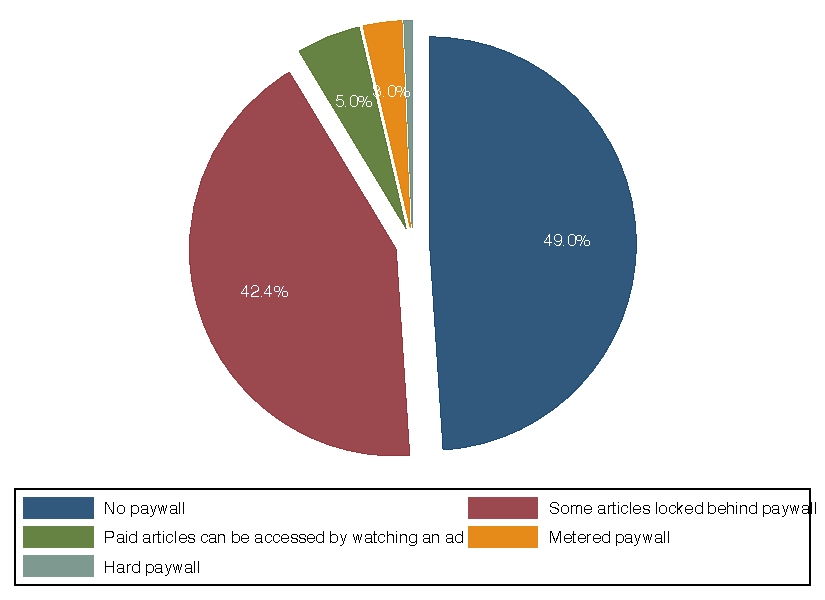
\includegraphics[scale=1]{figures/paywall_final}
\end{center}
	\begin{spacing}{0.5}
		{\footnotesize \textbf{Notes:} The Figure reports the share of the media outlets in our sample depending on their online business model. 48.1\% of the media in our sample do not have a paywall (``no paywall"), and $5.1\%$ condition the reading of the paid articles on the fact of watching an ad (``paid articles can be accessed by watching an ad"). Of the outlets that do have a paywall, we distinguish between three models: hard paywall, metered paywall, and soft paywall (``some articles locked behind paywall").}
	\end{spacing}
\vspace{.5cm}	
	\caption{News editors' business model}
	\label{fig:paywall_final}
\end{figure}
%%%%%%%%%%%%%%%%%%%%%%%%%%%%%%%%%%%%%%%%%%%%%%%%%%%%%%%%%%%%%%%%%%%%%% 


Third, given that media outlets may react differently to social media depending on their initial investment in quality \citep[see e.g.][]{deCorniereSarvary2019}, we also compute information on the size of the newsroom, and on the average payroll \citep{Cage2015_journalists}. This information is available for $68$ media outlets in our sample. Finally, for the $72$ media outlets for which this information is available, we collect daily audience information from the ACPM, the French press organization whose aim is to certify circulation and audience data. The average number of daily visitors is $588,722$, and the average number of page views $1,524,534$.


%%%%%%%%%%%%%%%%%%%%%%%%%%%%%%%%%
\subsubsection{Article characteristics}

Table \ref{Tab:sumstats_articles} presents summary statistics for the $929,764$ articles included in our dataset. On average, articles are $2,420$ characters long. For each of these articles, we also compute its originality rate, i.e. the share of the article that is ``original" and the share that is copy-pasted \citep{CageHerveViaud2020}.


%%%%%%%%%%%%%%%%%%%%%%%%%%%%%%%%%%%%%%%%%%%%%%%%%%%%%%%%%%%%%%%%%%%%%%
\begin{table}
\caption{Summary statistics: Mainstream media articles}
\begin{center}
	{
\def\sym#1{\ifmmode^{#1}\else\(^{#1}\)\fi}
\begin{tabular}{l*{1}{cccccc}}
\hline\hline
                    &\multicolumn{6}{c}{}                                                         \\
                    &        Mean&      St.Dev&         P25&      Median&         P75&         Max\\
\hline
\textbf{Length}     &            &            &            &            &            &            \\
Length (number of characters)&       2,420&       2,224&       1,125&       1,984&       3,184&     431,812\\
\textbf{Facebook shares}&            &            &            &            &            &            \\
Number of shares on Facebook&          19&         336&           0&           0&           1&      41,835\\
Number of comments on Facebook&          25&         308&           0&           0&           0&      19,316\\
Number of reactions on Facebook&          83&       1,535&        0.00&        0.00&        0.00&     200,136\\
\hline
Observations        &     929,764&            &            &            &            &            \\
\hline\hline
\end{tabular}
}

\end{center}
\begin{spacing}{0.5}
	{\fns \textbf{Notes:} The table gives summary statistics. Time period is July 2018-September 2018. Variables are values for the mainstream media articles. The observations are at the article level.} 
\end{spacing}
\label{Tab:sumstats_articles}
\end{table} 
%%%%%%%%%%%%%%%%%%%%%%%%%%%%%%%%%%%%%%%%%%%%%%%%%%%%%%%%%%%%%%%%%%%%%%



\medskip
In the remainder of this section, we describe the new algorithms we develop to analyze these two datasets, and in particular to identify the events on Twitter and investigate how they interact with mainstream media events.



%%%%%%%%%%%%%%%%%%%%%%%%%%%%%%%%%
\subsection{Detected events}
%%%%%%%%%%%%%%%%%%%%%%%%%%%%%%%%%

We use the method presented in Chapter \ref{Chap: Linking Media events and Twitter events}, Section \ref{JointEventsMethodo} to detect joint events in the corpus. We obtain $5,766$ joint events that encompass $28.4$ million tweets and $266,847$ news articles. Table \ref{Tab:table_summary_joint_events} presents summary statistics on these events that contain on average $4,924$ tweets and $46$ media articles published by $17$ media outlets. Of these $5,766$ joint events, $4,259$ break first on Twitter. These articles will be the focus of our analysis in Section \ref{Sec:EmpiricalSpecification} below. Their characteristics partly differ of those of the events that appear first on mainstream media, as reported in \hyperlink{ref:Appendix}{Appendix} Table \ref{Tab:table_summary_joint_events_ttest} where we perform a \textit{t}-test on the equality of means.


%%%%%%%%%%%%%%%%%%%%%%%%%%%%%%%%%%%%%%%%%%%%%%%%%%%%%%%%%%%%%%%%%%%%%%
\begin{table}
\caption{Summary statistics: Joint events\label{Tab:table_summary_joint_events}}
\begin{center}
{
\def\sym#1{\ifmmode^{#1}\else\(^{#1}\)\fi}
\begin{tabular}{l*{1}{cccccc}}
\hline\hline
                    &        Mean&      St.Dev&         P25&      Median&         P75&         Max\\
\hline
Length of the event (in hours)&         497&         493&         132&         290&         705&       2,319\\
Number of documents in event&       4,970&      72,423&         177&         590&       2,130&   5,253,528\\
\textbf{Twitter coverage}&            &            &            &            &            &            \\
Nb of tweets in event&       4,924&      72,383&         160&         556&       2,073&   5,250,923\\
Number of different Twitter users&       2,740&      15,575&         136&         461&       1,609&     956,814\\
Average number of retweets of tweets in events&         2.5&         4.6&         0.7&         1.4&         2.8&         120\\
Average number of replys of tweets in events&         0.3&         0.4&         0.1&         0.2&         0.4&          17\\
Average number of favorites of tweets in events&         3.6&         6.5&         0.7&         1.7&         4.0&         182\\
\textbf{Media coverage}&            &            &            &            &            &            \\
Number of news articles in the event&          46&         100&          13&          19&          41&       2,605\\
Number of different media outlets&          17&          11&           9&          13&          21&          98\\
\hline
Observations        &       5,766&            &            &            &            &            \\
\hline\hline
\end{tabular}
}

\end{center}
\begin{spacing}{0.5}
{\fns \textbf{Notes:} The table gives summary statistics. Time period is July 2018-September 2018. The observations are at the event level.}
\end{spacing}
\end{table} 
%%%%%%%%%%%%%%%%%%%%%%%%%%%%%%%%%%%%%%%%%%%%%%%%%%%%%%%%%%%%%%%%%%%%%%


%%%%%%%%%%%%%%%%%%%%%%%%%%%%%%%%%

There are several reasons why an event may appear on Twitter first, before being covered by mainstream media. First, an event may be described by a media outlet outside of our corpus, such as an English-language news agency, then be picked up by Twitter users before being relayed by the French media. Second, some Twitter users can witness a ``real world" event and film it or talk about it on social networks. This was the case with ``the battle of Orly airport", when French rappers Booba and Kaaris got into a fight inside a duty-free store in 2018. Third, some events may originate solely on Twitter, such as the accusations that certain French Youtube influencers had raped minors. These allegations spread in August 2018 with the hashtag \#BalanceTonYoutubeur.



%%%%%%%%%%%%%%%%%%%%%%%%%%%%%%%%%
\subsection{Measures of popularity on Twitter and of media coverage}
%%%%%%%%%%%%%%%%%%%%%%%%%%%%%%%%%

To proxy the popularity of an event on Twitter, we rely on the activity on Twitter and count, in each event, the total number of tweets and the total number of unique users who tweet about the event. For the tweets, we distinguish between the original tweets and the retweets and replies. Furthermore, we compute the average number of followers of the news breaker or seed of the event.

Importantly, to isolate the specific impact of the popularity of a Twitter event $e_T$ on mainstream media coverage we focus on what happens on social media \textit{before} the publication of the first news article; to do so, we compute similar measures but focus only on Twitter activity before the first mainstream media article appears. In the IV strategy described below (Section \ref{Sec:SpecificationIV}), to instrument for this popularity, we also compute the average number of interactions generated by the seed's previous tweets, as well as the interactions generated by the tweets of the seeds' followers.\footnote{To compute this number of interactions, we also include in our dataset of tweets the period between June 15th 2018 and June 30th 2018. We do so to ensure that we observe at least some tweets before the first event.} 


To study the intensity of mainstream media coverage, we look at different dimensions. First, we use quantitative measures of coverage, in particular the number of articles a given media outlet devotes to the event, as well as the length of these articles. Studying both the intensive and the extensive margin of coverage is of particular importance here given that some media outlets can choose to skip some events while others may decide to follow a more systematic approach. This may depend on the characteristics of the media outlet, but also on the topic of the event.

Second, we use more ``qualitative" measures of coverage, in particular the originality of the articles \citep[following][]{CageHerveViaud2020} and the ``reactivity" of the media (i.e. the time it takes the media to cover the event, with respect to both the other media outlets and the beginning of the SMEs).


%%%%%%%%%%%%%%%%%%%%%%%%%%%%%%%%%%%%%%%%%%%%%%%%%%%%%%%%%%%%%%%%
%%%%%%%%%%%%%%%%%%%%%%%%%%%%%%%%%%%%%%%%%%%%%%%%%%%%%%%%%%%%%%%%
\section{Popularity on Twitter and news editor decisions: Empirical strategy\label{Sec:EmpiricalSpecification}}
%%%%%%%%%%%%%%%%%%%%%%%%%%%%%%%%%%%%%%%%%%%%%%%%%%%%%%%%%%%%%%%%
%%%%%%%%%%%%%%%%%%%%%%%%%%%%%%%%%%%%%%%%%%%%%%%%%%%%%%%%%%%%%%%%

In the remainder of this chapter, we tackle the following question: does the popularity of a story on social media affect, everything else equal, the coverage that mainstream media devote to this story? While the drivers of news editors' decisions remain essentially a black box, understanding the role played by social media in these decisions is of particular importance. In this Section, we present the empirical strategy we develop to tackle this question; the empirical results are presented in the following Section \ref{Sec:Results}.


%%%%%%%%%%%%%%%%%%%%%%%%%%%%%%%%%
\subsection{Naive approach\label{Sec:SpecificationOLS}}
%%%%%%%%%%%%%%%%%%%%%%%%%%%%%%%%%

We begin by estimating the correlation between an event popularity on Twitter and its mainstream media coverage. We do so both at the event level and the media level.


%%%%%%%%%%%%%%%%%%%%%%%%%%%%%%%%%
\paragraph{Event-level approach}

At the event-level, we perform the following estimation:

\begin{equation}
\mathtt{coverage}_{e}= \alpha + \mathbf{Z'_{e}}\beta + \lambda_d + \omega_m + \epsilon_{emd}
\label{eq:OLSevent}
\end{equation}

\noindent  where $e$ index the events, $d$ the day of the week (DoW) of the first tweet in the event, and $m$ the month.

Our dependent variable of interest, $\mathtt{coverage}_{e}$, is the intensity of the media coverage that we proxy at the event level by the total number of articles devoted to the event and the number of different media outlets covering the event. Our main explanatory variable, $\mathbf{Z'_{e}}$, is a  vector that captures the popularity of the event on Twitter \textit{before} the publication of the first article. This vector includes alternatively the total number of tweets in the event and the number of original tweets, retweets and replies. We always control for the seed's number of followers (at the time of the event). We also control for DoW fixed effects ($\lambda_d$) and month fixed effects ($\omega_m$). Given that the dependent variable is a count variable, we use a negative binomial to estimate equation~(\ref{eq:OLSevent}).
%\footnote{In the online Appendix Section \ref{Sec:Robustness}, we show that our results are robust to the use of different specifications.} 
%  as well as the average audience of these tweets (measured by their number of retweets, likes, and quotes)


%%%%%%%%%%%%%%%%%%%%%%%%%%%%%%%%%
\paragraph{Media-level approach}

Bias in editorial decisions may vary depending on the characteristics of the media outlet. Furthermore, some media outlets may decide to cover a news event while others do not. To investigate whether this is the case, we then exploit within media outlet variations (in this case, the standard errors are clustered at the event level). Our specification is as follows: 

\begin{equation}
\mathtt{coverage}_{ec}= \alpha + \mathbf{Z'_{e}}\beta +  \delta_{c}  + \lambda_d + \omega_m +\epsilon_{ecmd}
\label{eq:OLSmedia}
\end{equation}

\noindent where $c$ index the media outlets and the dependent variable, $\mathtt{coverage}_{ec}$, is now alternatively the number of articles published by media $c$ in event $e$ and, conditional on covering the event, the average length and originality of these articles, and the reactivity of the media. $\mathbf{Z'_{e}}$ is the same vector as in equation~(\ref{eq:OLSevent}) and measures the popularity of the event on Twitter. $\delta_{c}$,  $\lambda_d$ and $\omega_m$ are respectively fixed effects for media, DoW and month.



%%%%%%%%%%%%%%%%%%%%%%%%%%%%%%%%%
\subsection{IV approach\label{Sec:SpecificationIV}}
%%%%%%%%%%%%%%%%%%%%%%%%%%%%%%%%%

While estimating equations~(\ref{eq:OLSevent}) and (\ref{eq:OLSmedia}) allows us to analyze the relationship between the popularity of a story on Twitter and its coverage on mainstream media, the estimated relationship may be (at least partly) driven by the unobserved characteristics of the story, e.g. its ``newsworthiness". Randomizing story popularity on Twitter is not feasible. To identify the causal effect of a popularity shock on Twitter, we thus need to find and exploit exogenous sources of variation in popularity. We propose a new IV strategy that relies on the structure of the Twitter network interacted with ``news pressure" at the time of the event.

When exploiting the structure of the Twitter network, the intention of our identification strategy approach is to mimic a hypothetical experiment that would break the correlation between popularity and unobserved determinants of the story's intrinsic interest. Our source of exogenous variation, in the spirit of an intention-to-treat approach, comes from the number of ``impressions" generated by the user's previous tweets. The intuition here is as follows: everything else equal and regardless of the interest of a given tweet, the higher the number of impressions, the higher the potential number of retweets. More precisely, for all the seeds of the events, we compute the number of interactions generated by their \textit{previous} tweets (i.e. before the beginning of the event). We drop the events whose seed is the Twitter account of a media outlet or journalist, as well as the events which are broken by Twitter accounts that broke more than one event during our time period (multiple news breaker) to avoid capturing a celebrity or influencer bias, and we control for the seed's number of followers.

We then go one step further: rather than computing the interactions generated by the seed's previous tweets, we compute the interactions of the previous tweets of the seed's followers in the spirit of Figure \ref{fig:follower} presented in the introduction. The idea here is to establish that, for two ``similar" seeds as defined by their number of followers, everything else equal, the tweets of the seed whose followers themselves have a high number of followers will generate more impressions -- and so have a higher probability of being retweeted -- than the same tweets by the seed whose followers have just a few followers. However, while presumably more exogenous than the previous approach, the number of interactions generated by the seeds' followers may still suffer from the fact that a seed's centrality in the Twitter network may be related to its ability to produce newsworthy content. 

To relax the exclusion restriction, the instrument we propose here is the interaction between the seed's centrality in the network (as previously defined) and the news pressure at the time of the tweet, controlling for the direct effect of centrality and news pressure. We measure news pressure by the number of interactions generated by all the tweets published in the hour preceding the first tweet in the event. The idea, in the spirit of \citet{EisenseeStromberg2007}, is that, if at the time of the first tweet in the event there are some very popular tweets, then those tweets generate a crowding-out effect: given that they receive a high number of retweets/replies/quotes, they ``overfill" the Twitter feed and make the first tweet in the event less visible, regardless of its newsworthiness. In other words, if two equally newsworthy stories are covered on Twitter, we would expect that the story occurring when there is a high number of other stories around would have a lower chance of receiving a large number of retweets than the story occurring when there is little activity on Twitter (controlling for the time of the day). We measure the total number of reactions (retweets/replies/quotes) rather than the total number of tweets, because the Twitter API may restrict the number of delivered tweets if it exceeds the threshold of 1\% of the global volume. The number of retweets, on the other hand, is known at any time because it is a metadata provided with each tweet. Figure \ref{fig:news_pressure_hour_illustration} illustrates our IV strategy: for each minute, we compute the average number of interactions generated by the tweets published during the previous hour. It is clear that there are many variations in this number.


%%%%%%%%%%%%%%%%%%%%%%%%%%%%%%%%%%%%%%%%%%%%%%%%%%%%%%%%%%%%%%%%%%%%%%
\begin{figure}
\begin{center}
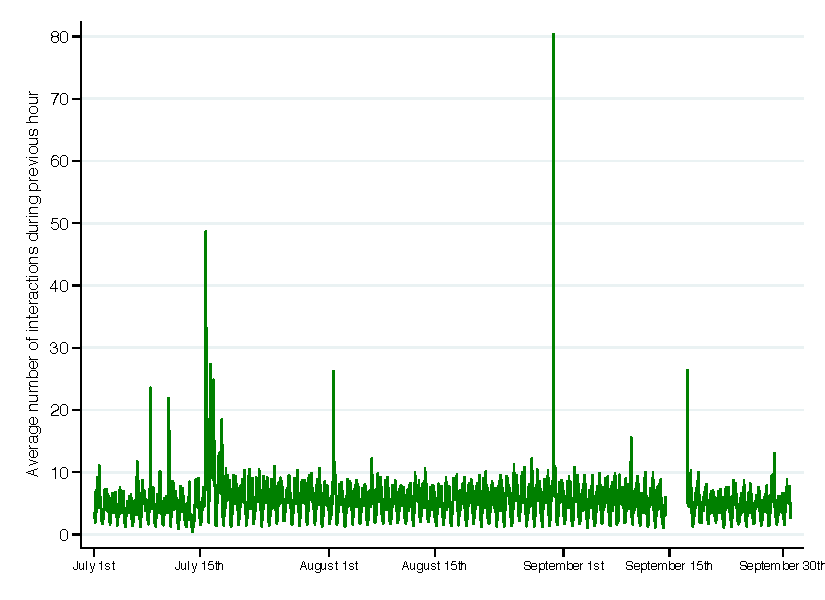
\includegraphics[scale=1]{figures/news_pressure_hour_illustration}
\end{center}
	\begin{spacing}{0.5}
		{\footnotesize \textbf{Notes:} The Figure reports the average number of interactions (retweets/replies/favorites) generated by the tweets published during the previous hour. The average number of interactions is computed at the minute level.}
	\end{spacing}
\vspace{.5cm}	
	\caption{News pressure: Average number of interactions generated by the tweets published during the previous hour}
	\label{fig:news_pressure_hour_illustration}
\end{figure}
%%%%%%%%%%%%%%%%%%%%%%%%%%%%%%%%%%%%%%%%%%%%%%%%%%%%%%%%%%%%%%%%%%%%%% 

 
News pressure alone cannot be a reliable instrument, however: it can indeed affect both Twitter and the media at the same time. This is why our instrument is the interaction between news pressure and centrality in the network as previously defined. Our identification assumption is that, once we control for the direct effects of centrality and news pressure, the interaction between the seed's centrality and news pressure should only affect traditional news production through its effect on the tweet's visibility on Twitter. This is conditional on controlling for the seed's number of followers and, as highlighted above, dropping the events whose seed is the Twitter account of a media outlet or journalist and/or whose seed is a multiple news breaker.



%%%%%%%%%%%%%%%%%%%%%%%%%%%%%%%%%%%%%%%%%%%%%%%%%%%%%%%%%%%%%%%%
%%%%%%%%%%%%%%%%%%%%%%%%%%%%%%%%%%%%%%%%%%%%%%%%%%%%%%%%%%%%%%%%
\section{Popularity on social media and news editor decisions: Results\label{Sec:Results}}
%%%%%%%%%%%%%%%%%%%%%%%%%%%%%%%%%%%%%%%%%%%%%%%%%%%%%%%%%%%%%%%%
%%%%%%%%%%%%%%%%%%%%%%%%%%%%%%%%%%%%%%%%%%%%%%%%%%%%%%%%%%%%%%%%

In this Section, we first present the results of the naive estimations (without instrumenting for event popularity). We then turn to the IV analysis before discussing the heterogeneity of the effects.


%%%%%%%%%%%%%%%%%%%%%%%%%%%%%%%%%
\subsection{Naive estimates}

%%%%%%%%%%%%%%%%%%%%%%%%%%%%%%%%%
\paragraph{Event-level analysis}

Table \ref{Tab:number_articles_negbinomial_event} reports the results of the estimation of equation~(\ref{eq:OLSevent}) (event-level analysis). In Columns (1) to (4) the outcome of interest is the total number of articles published in the event, and in Columns (5) and (6) the number of unique media outlets which cover the event. As highlighted above, given that these dependent variables are count variables, we use a negative binomial. We find a positive correlation between the number of tweets published in an event before the first news article (``number of tweets") and the total number of articles published in the event: an increase of $1,000$ in the number of tweets published in the event before the first media article is associated with $2.3$ additional articles (Column (1)); this finding is robust to dropping the events whose seed is the Twitter account of a media outlet or journalist and the events whose seed is the Twitter account of a multiple news breaker (as defined above). Doing so only slightly decreases the magnitude of the relationship (Column (3)). What is more, this effect is mainly driven by the number of original tweets in the event; the number of retweets and replies do not have a positive effect (Columns (2) and (4)).

The positive relationship between the popularity of the event on Twitter and the media coverage is driven both by the intensity of the coverage (number of articles) and by the extensive margin: we also find a positive relationship with the number of unique media outlets covering the event (Columns (5) and (6)). An increase of 1,000 in the number of original tweets published in the event before the first media article is associated with an increase of $1.3$ in the number of media outlets dealing with the event.


%%%%%%%%%%%%%%%%%%%%%%%%%%%%%%%%%%%%%%%%%%%%%%%%%%%%%%%%%%%%%%%%%%%%%%
\begin{table}
\caption{Naive estimates: Event-level approach}
\begin{center}
	{
\def\sym#1{\ifmmode^{#1}\else\(^{#1}\)\fi}
\begin{tabular}{l*{6}{c}}
\hline\hline
                    &\multicolumn{4}{c}{Number of articles}                                                 &\multicolumn{2}{c}{Number of media}        \\\cmidrule(lr){2-5}\cmidrule(lr){6-7}
                    &\multicolumn{1}{c}{(1)}         &\multicolumn{1}{c}{(2)}         &\multicolumn{1}{c}{(3)}         &\multicolumn{1}{c}{(4)}         &\multicolumn{1}{c}{(5)}         &\multicolumn{1}{c}{(6)}         \\
\hline
main                &                     &                     &                     &                     &                     &                     \\
Number of tweets    &       0.052\sym{***}&                     &       0.043\sym{***}&                     &       0.020\sym{***}&                     \\
                    &     (0.013)         &                     &     (0.010)         &                     &     (0.004)         &                     \\
Number of original tweets&                     &       0.517\sym{***}&                     &       0.394\sym{***}&                     &       0.079\sym{*}  \\
                    &                     &     (0.125)         &                     &     (0.132)         &                     &     (0.044)         \\
Number of retweets  &                     &      -0.005         &                     &       0.005         &                     &       0.016\sym{***}\\
                    &                     &     (0.009)         &                     &     (0.011)         &                     &     (0.006)         \\
Number of replies   &                     &      -0.331\sym{**} &                     &      -0.262\sym{*}  &                     &      -0.062         \\
                    &                     &     (0.161)         &                     &     (0.158)         &                     &     (0.092)         \\
Seed's number of followers&       0.000         &       0.000         &      -0.000         &      -0.000         &       0.000         &       0.000         \\
                    &     (0.000)         &     (0.000)         &     (0.000)         &     (0.000)         &     (0.000)         &     (0.000)         \\
\hline
Month \& DoW FEs    &  \checkmark         &  \checkmark         &  \checkmark         &  \checkmark         &  \checkmark         &  \checkmark         \\
Drop media          &                     &                     &  \checkmark         &  \checkmark         &  \checkmark         &  \checkmark         \\
Drop multiple       &                     &                     &  \checkmark         &  \checkmark         &  \checkmark         &  \checkmark         \\
Observations        &       4,259         &       4,259         &       3,163         &       3,163         &       3,163         &       3,163         \\
Marginal Effect (tweets)&         2.3         &                     &         1.8         &                     &         0.3         &                     \\
Marginal Effect (original tweets)&                     &        31.2         &                     &        18.2         &                     &         1.3         \\
\hline\hline
\end{tabular}
}

\end{center}
\begin{spacing}{0.5}
	{\fns \textbf{Notes:} * p$<$0.10, ** p$<$0.05, *** p$<$0.01. The time period is July 2018-September 2018.  Models are estimated using a negative binomial estimation (robust standard errors are reported between parentheses). An observation is a news event. We only consider the subset of news events that appear first on Twitter. All specifications include the seed's number of followers as a control, and day-of-the-week and month fixed effects. Columns (1) and (2) report the estimates for all the events that appear first on Twitter; in Columns (3) to (6) we drop the events whose seed is the Twitter account of a media outlet or journalist (``media") as well as the events whose seed broke more than one event during our time period (``multiple"). The independent variables (number of tweets, number of original tweets, etc.) are computed \textit{before} the first news article in the event and are given in thousands. More details are provided in the text.} 
\end{spacing}
\label{Tab:number_articles_negbinomial_event}
\end{table} 
%%%%%%%%%%%%%%%%%%%%%%%%%%%%%%%%%%%%%%%%%%%%%%%%%%%%%%%%%%%%%%%%%%%%%%


%%%%%%%%%%%%%%%%%%%%%%%%%%%%%%%%%
\paragraph{Media-level analysis}

Table \ref{Tab:number_articles_negbinomial_cevent} shows the estimates when we perform the media-level analysis (estimation of equation~(\ref{eq:OLSmedia})). The unit of observation is a media-event, and all the media outlets are included in the estimation (even if they do not cover the event; then the value of the number of articles in the event for them is equal to zero). Consistently with the results in Table \ref{Tab:number_articles_negbinomial_event}, we find a positive relationship between the popularity of the event on Twitter and the media coverage it receives (Column (1)), and this relationship is robust to dropping the events whose seed is the Twitter account of a media / journalist / multiple news breaker (Column (2)). An increase of $1,000$ in the number of tweets published in the event before the first media article appears increases the average number of articles that \textit{each media outlet} publishes in the event by $0.011$. 

In Columns (3) to (6) we investigate whether this relationship varies with the media characteristics, and in particular with the intensity of their social media presence. We define this intensity here with respect to the share of the media outlet's articles that are published on social media. We find that the strength of the relationship is higher for the outlets whose social media presence is high than for the media whose social media presence is relatively lower. We will come back to this finding when discussing the mechanisms at play in Section \ref{Sec:Mechanisms} below. We then investigate whether these effects depend on the offline format of the media. Table \ref{Tab:number_articles_negbinomial_cevent_heterogeneity} presents the results. While we observe a positive and statistically significant relationship for all the media outlets, the magnitude is the strongest for the websites of the television stations.
% JULIA: A RAJOUTER PLUS TARD Robustness avec les autres mesures de social media presence (e.g. number of Twitter accounts)


%%%%%%%%%%%%%%%%%%%%%%%%%%%%%%%%%%%%%%%%%%%%%%%%%%%%%%%%%%%%%%%%%%%%%%
\begin{sidewaystable}
\caption{Naive estimates: Media-level approach}
\begin{center}
	{
\def\sym#1{\ifmmode^{#1}\else\(^{#1}\)\fi}
\begin{tabular}{l*{6}{c}}
\hline\hline
                    &\multicolumn{2}{c}{All}                    &\multicolumn{2}{c}{Low social media presence}&\multicolumn{2}{c}{High social media presence}\\\cmidrule(lr){2-3}\cmidrule(lr){4-5}\cmidrule(lr){6-7}
                    &\multicolumn{1}{c}{(1)}         &\multicolumn{1}{c}{(2)}         &\multicolumn{1}{c}{(3)}         &\multicolumn{1}{c}{(4)}         &\multicolumn{1}{c}{(5)}         &\multicolumn{1}{c}{(6)}         \\
\hline
Number of articles  &                     &                     &                     &                     &                     &                     \\
Number of tweets    &       0.048\sym{***}&       0.041\sym{***}&       0.042\sym{***}&       0.038\sym{***}&       0.050\sym{***}&       0.042\sym{***}\\
                    &     (0.009)         &     (0.008)         &     (0.009)         &     (0.008)         &     (0.010)         &     (0.008)         \\
Seed's number of followers&       0.000         &      -0.000         &       0.000\sym{*}  &      -0.000         &       0.000         &      -0.000         \\
                    &     (0.000)         &     (0.000)         &     (0.000)         &     (0.000)         &     (0.000)         &     (0.000)         \\
\hline
Media FEs           &  \checkmark         &  \checkmark         &  \checkmark         &  \checkmark         &  \checkmark         &  \checkmark         \\
Month \& DoW FEs    &  \checkmark         &  \checkmark         &  \checkmark         &  \checkmark         &  \checkmark         &  \checkmark         \\
Drop media          &                     &  \checkmark         &                     &  \checkmark         &                     &  \checkmark         \\
Drop multiple       &                     &  \checkmark         &                     &  \checkmark         &                     &  \checkmark         \\
Observations        &     800,692         &     594,644         &     400,346         &     297,322         &     400,346         &     297,322         \\
Clusters (events)   &       4,259         &       3,163         &       4,259         &       3,163         &       4,259         &       3,163         \\
Marginal Effect     & {0.011}             &     0.009           & {0.007}             &       0.006         & {0.015}             &       0.012        \\
\hline\hline
\end{tabular}
}

\end{center}
\begin{spacing}{0.5}
	{\fns \textbf{Notes:} * p$<$0.10, ** p$<$0.05, *** p$<$0.01. The time period is July 2018 - September 2018.  Models are estimated using a negative binomial estimation. Standard errors are clustered at the event level. An observation is a media-news event. We only consider the subset of news events that appear first on Twitter. All specifications include the seed's number of followers as a control, and day-of-the-week, month, and media fixed effects. Columns (1), (3) and (5) report the estimates for all the events that appear first on Twitter; in Columns (2), (4) and (6) we drop the events whose seed is the Twitter account of a media or of journalist (``media") as well as the events whose seed broke more than one event during our time period (``multiple"). In Columns (1) and (2) all the media outlets in our sample are included; in Columns (3) and (4) (respectively Columns (5) and (6)) we only consider the media outlets whose social media presence is low (respectively high). High and low social media presence are defined by the share of the media outlet's articles published on social media (above or below the median). The number of tweets is computed \textit{before} the first news article in the event and is in thousand. More details are provided in the text.} 
\end{spacing}
\label{Tab:number_articles_negbinomial_cevent}
\end{sidewaystable} 
%%%%%%%%%%%%%%%%%%%%%%%%%%%%%%%%%%%%%%%%%%%%%%%%%%%%%%%%%%%%%%%%%%%%%%


%%%%%%%%%%%%%%%%%%%%%%%%%%%%%%%%%%%%%%%%%%%%%%%%%%%%%%%%%%%%%%%%%%%%%%
\begin{table}
\caption{Naive estimates: Media-level approach, Depending on the media offline format}
\begin{center}
	{
\def\sym#1{\ifmmode^{#1}\else\(^{#1}\)\fi}
\begin{tabular}{l*{6}{c}}
\hline\hline
                    &\multicolumn{1}{c}{Nat. dail.}&\multicolumn{1}{c}{Local dail.}&\multicolumn{1}{c}{Weeklies}&\multicolumn{1}{c}{Pure online}&\multicolumn{1}{c}{TV}&\multicolumn{1}{c}{Radio}\\\cmidrule(lr){2-2}\cmidrule(lr){3-3}\cmidrule(lr){4-4}\cmidrule(lr){5-5}\cmidrule(lr){6-6}\cmidrule(lr){7-7}
                    &\multicolumn{1}{c}{(1)}         &\multicolumn{1}{c}{(2)}         &\multicolumn{1}{c}{(3)}         &\multicolumn{1}{c}{(4)}         &\multicolumn{1}{c}{(5)}         &\multicolumn{1}{c}{(6)}         \\
\hline
Number of articles  &                     &                     &                     &                     &                     &                     \\
Number of tweets    &       0.033\sym{***}&       0.039\sym{***}&       0.042\sym{***}&       0.048\sym{***}&       0.059\sym{***}&       0.039\sym{***}\\
                    &     (0.009)         &     (0.008)         &     (0.008)         &     (0.009)         &     (0.013)         &     (0.009)         \\
Seed's number of followers&      -0.000\sym{**} &      -0.000         &      -0.000         &       0.000         &      -0.000         &      -0.000         \\
                    &     (0.000)         &     (0.000)         &     (0.000)         &     (0.000)         &     (0.000)         &     (0.000)         \\
\hline
Media FEs           &  \checkmark         &  \checkmark         &  \checkmark         &  \checkmark         &  \checkmark         &  \checkmark         \\
Month \& DoW FEs    &  \checkmark         &  \checkmark         &  \checkmark         &  \checkmark         &  \checkmark         &  \checkmark         \\
Drop media          &  \checkmark         &  \checkmark         &  \checkmark         &  \checkmark         &  \checkmark         &  \checkmark         \\
Drop multiple       &  \checkmark         &  \checkmark         &  \checkmark         &  \checkmark         &  \checkmark         &  \checkmark         \\
Observations        &      34,793         &      88,564         &     107,542         &     205,595         &      22,141         &      34,793         \\
Clusters (events)   &       3,163         &       3,163         &       3,163         &       3,163         &       3,163         &       3,163         \\
Marginal Effect     &       0.017         &       0.012         &       0.009         &       0.003         &       0.020         &       0.013         \\
\hline\hline
\end{tabular}
}

\end{center}
\begin{spacing}{0.5}
	{\fns \textbf{Notes:} * p$<$0.10, ** p$<$0.05, *** p$<$0.01. The time period is July 2018-September 2018.  Models are estimated using a negative binomial estimation. Standard errors are clustered at the event level. An observation is a media-news event. We only consider the subset of news events that appear first on Twitter, and drop the events whose seed is the Twitter account of a media outlet or journalist (``media") as well as the events whose seed broke more than one event during our time period (``multiple"). All specifications include the seed's number of followers as a control, and day-of-the-week, month, and media fixed effects. In Column (1), we only consider the national daily newspapers, in Column (2) the local daily newspapers, in Column (3) the weekly newspapers, in Column (4) the pure online media, in Column (5) the television channel websites, and in Column (6) the radio station websites. The number of tweets is computed \textit{before} the first news article in the event appears and is given in thousands. More details are provided in the text.} 
\end{spacing}
\label{Tab:number_articles_negbinomial_cevent_heterogeneity}
\end{table} 
%%%%%%%%%%%%%%%%%%%%%%%%%%%%%%%%%%%%%%%%%%%%%%%%%%%%%%%%%%%%%%%%%%%%%%


%%%%%%%%%%%%%%%%%%%%%%%%%%%%%%%%%%%%%%%%%%%%%%%%%%%%%%%%%%%%%%%%%%%%%
% POUR L'INSTANT ON NE MONTRE PAS CETTE TABLE -- PEUT-ETRE APRES L'IV
%\begin{sidewaystable}
%\caption{Naive estimates: Media-level approach, Depending on the offline format}
%\begin{center}
%	{
\def\sym#1{\ifmmode^{#1}\else\(^{#1}\)\fi}
\begin{tabular}{l*{8}{c}}
\hline\hline
                    &\multicolumn{2}{c}{No paywall}             &\multicolumn{2}{c}{Paywall}                &\multicolumn{2}{c}{Small newsroom}         &\multicolumn{2}{c}{Large newsroom}         \\\cmidrule(lr){2-3}\cmidrule(lr){4-5}\cmidrule(lr){6-7}\cmidrule(lr){8-9}
                    &\multicolumn{1}{c}{(1)}         &\multicolumn{1}{c}{(2)}         &\multicolumn{1}{c}{(3)}         &\multicolumn{1}{c}{(4)}         &\multicolumn{1}{c}{(5)}         &\multicolumn{1}{c}{(6)}         &\multicolumn{1}{c}{(7)}         &\multicolumn{1}{c}{(8)}         \\
\hline
Number of articles  &                     &                     &                     &                     &                     &                     &                     &                     \\
Number of tweets    &       0.051\sym{***}&       0.045\sym{***}&       0.044\sym{***}&       0.036\sym{***}&       0.044\sym{***}&       0.038\sym{***}&       0.052\sym{***}&       0.041\sym{***}\\
                    &     (0.008)         &     (0.008)         &     (0.011)         &     (0.008)         &     (0.010)         &     (0.009)         &     (0.013)         &     (0.009)         \\
Seed's number of followers&       0.000         &       0.000         &       0.000         &      -0.000\sym{*}  &       0.000\sym{*}  &      -0.000         &       0.000\sym{*}  &      -0.000         \\
                    &     (0.000)         &     (0.000)         &     (0.000)         &     (0.000)         &     (0.000)         &     (0.000)         &     (0.000)         &     (0.000)         \\
\hline
Media FEs           &  \checkmark         &  \checkmark         &  \checkmark         &  \checkmark         &  \checkmark         &  \checkmark         &  \checkmark         &  \checkmark         \\
Month \& DoW FEs    &  \checkmark         &  \checkmark         &  \checkmark         &  \checkmark         &  \checkmark         &  \checkmark         &  \checkmark         &  \checkmark         \\
Drop media          &                     &  \checkmark         &                     &  \checkmark         &                     &  \checkmark         &                     &  \checkmark         \\
Drop multiple       &                     &  \checkmark         &                     &  \checkmark         &                     &  \checkmark         &                     &  \checkmark         \\
Observations        &     472,749         &     351,093         &     264,058         &     196,106         &     140,547         &     104,379         &     144,806         &     107,542         \\
Clusters (events)   &       4,259         &       3,163         &       4,259         &       3,163         &       4,259         &       3,163         &       4,259         &       3,163         \\
Marginal Effect     &       0.011         &       0.010         &       0.013         &       0.010         &       0.010         &       0.008         &       0.047         &       0.034         \\
\hline\hline
\end{tabular}
}

%\end{center}
%\begin{spacing}{0.5}
%	{\fns \textbf{Notes:} \textbf{REPRENDRE}} 
%\end{spacing}
%\label{Tab:number_articles_negbinomial_cevent_heterogeneity_paywall_journalists}
%\end{sidewaystable} 
%%%%%%%%%%%%%%%%%%%%%%%%%%%%%%%%%%%%%%%%%%%%%%%%%%%%%%%%%%%%%%%%%%%%%%


Next, we focus on the media outlets that devote at least one article to the event and investigate the magnitude of the coverage, \textit{conditional on covering} the event. Indeed, the popularity of an event on Twitter can indeed play a role both at the intensive and at the extensive margin. Table \ref{Tab:number_articles_negbinomial_Dcover_cevent} presents the results. Columns (1) and (2) present the estimations for the number of articles published by the media in the event: we see that the positive impact of popularity appears not only at the extensive margin but also at the intensive margin given that there is a positive correlation with the number of articles published (conditional on publishing at least one article in the event). However, the magnitude of this relationship is weak: an increase of $1,000$ increase in the number of tweets is associated with an increase of $0.05$ in the number of articles published by each media outlet.

In addition, we find a statistically significant relationship with the length of the article(s) published by the media (Columns (3) and (4)). The length of the articles can be considered a proxy -- albeit an imperfect one -- for the quality of the articles. We will come back to this point in the mechanisms section below.


%%%%%%%%%%%%%%%%%%%%%%%%%%%%%%%%%%%%%%%%%%%%%%%%%%%%%%%%%%%%%%%%%%%%%%
\begin{table}
\caption{Naive estimates: Media-level approach, Conditional on covering the event}
\begin{center}
	{
\def\sym#1{\ifmmode^{#1}\else\(^{#1}\)\fi}
\begin{tabular}{l*{4}{c}}
\hline\hline
                    &\multicolumn{2}{c}{Number of articles}     &\multicolumn{2}{c}{Articles length}        \\\cmidrule(lr){2-3}\cmidrule(lr){4-5}
                    &\multicolumn{1}{c}{(1)}         &\multicolumn{1}{c}{(2)}         &\multicolumn{1}{c}{(3)}         &\multicolumn{1}{c}{(4)}         \\
\hline
main                &                     &                     &                     &                     \\
Number of tweets    &        0.02\sym{***}&        0.02\sym{***}&        7.58\sym{***}&        7.64\sym{***}\\
                    &      (0.01)         &      (0.00)         &      (2.38)         &      (2.51)         \\
Seed's number of followers&        0.00         &       -0.00\sym{*}  &        0.00         &       -0.00         \\
                    &      (0.00)         &      (0.00)         &      (0.00)         &      (0.00)         \\
\hline
Media FEs           &  \checkmark         &  \checkmark         &  \checkmark         &  \checkmark         \\
Month \& DoW FEs    &  \checkmark         &  \checkmark         &  \checkmark         &  \checkmark         \\
Drop media          &                     &  \checkmark         &                     &  \checkmark         \\
Drop multiple       &                     &  \checkmark         &                     &  \checkmark         \\
R-sq (within)       &                     &                     &       0.001         &       0.001         \\
Observations        &      70,133         &      52,246         &      70,124         &      52,237         \\
Clusters (events)   &       4,259         &       3,163         &       4,259         &       3,163         \\
Marginal Effect     &        0.05         &        0.04         &                     &                     \\
\hline\hline
\end{tabular}
}

\end{center}
\begin{spacing}{0.5}
	{\fns \textbf{Notes:} * p$<$0.10, ** p$<$0.05, *** p$<$0.01. The time period is July 2018-September 2018.  Models are estimated using a negative binomial estimation in Columns (1) and (2), and OLS in Columns (3) to (4). Standard errors are clustered at the event level. An observation is a media-news event, and only the media outlets that devote at least one article to the event are included. Furthermore, we only consider the subset of news events that appear first on Twitter. All specifications include the seed's number of followers as a control, and day-of-the-week, month, and media fixed effects. Columns (1) and (3) report the estimates for all the events that appear first on Twitter; in Columns (2) and (4) we drop the events whose seed is the Twitter account of a media outlet or journalist (``media") as well as the events whose seed broke more than one event during our time period (``multiple"). In Columns (1) and (2), the dependent variable is the number of articles published by the media outlet; in Columns (3) and (4) the average length of these articles. The number of tweets is computed \textit{before} the first news article in the event appears and is given in thousands. More details are provided in the text.}
% , and in Columns (5) and (6) the reaction time in hours (we take the minimum reaction time when the media publishes more than one article in the event)	
\end{spacing}
\label{Tab:number_articles_negbinomial_Dcover_cevent}
\end{table} 
%%%%%%%%%%%%%%%%%%%%%%%%%%%%%%%%%%%%%%%%%%%%%%%%%%%%%%%%%%%%%%%%%%%%%%



%%%%%%%%%%%%%%%%%%%%%%%%%%%%%%%%%
\subsection{IV estimates\label{Sec:ResultsIV}}
%%%%%%%%%%%%%%%%%%%%%%%%%%%%%%%%%

The previous estimates may suffer from the fact that the positive relationship between a story's popularity on Twitter and its media coverage can both be driven by the intrinsic interest of the story, regardless of what happens on social media. Hence, in this section, we report the results of the IV estimates following the strategy described in Section \ref{Sec:SpecificationIV} above.

Table \ref{Tab:number_articles_IV} reports the results of the estimation. In Columns (1) and (2) we report the results of the first stage (the dependent variable is the number of tweets before the number of articles in the event) and in Columns (3) and (4) the second, where the main explanatory variable, number of tweets, is instrumented by the interaction between news pressure and centrality in the network. As can be clearly seen from Columns (1) and (2), our instrument ``High pressure * Previous interactions" has a statistically significant effect on the number of tweets in the event. Second, we find that there is a positive and statistically significant causal effect of the number of tweets on the number of articles (Columns (3) and (4)). This effect is robust to dropping the events whose seed is the Twitter account of a media outlet / journalist / multiple news breaker (as previously defined).

Regarding the magnitude of the effects, we find that an increase of $1,000$ in the number of tweets is associated with an increase of $1.11$ in the number of articles published in the event. Hence the magnitude of the IV estimates is around half that of the naive estimates. This is consistent with the expected direction of the bias given that the unobserved newsworthiness of events should drive upward both the number of articles and the number of tweets in the event.


%%%%%%%%%%%%%%%%%%%%%%%%%%%%%%%%%%%%%%%%%%%%%%%%%%%%%%%%%%%%%%%%%%%%%%
\begin{table}
\caption{IV estimates: Media-level approach}
\begin{center}
	{
\def\sym#1{\ifmmode^{#1}\else\(^{#1}\)\fi}
\begin{tabular}{l*{4}{c}}
\hline\hline
                    &\multicolumn{2}{c}{Number of tweets}       &\multicolumn{2}{c}{Number of articles}     \\\cmidrule(lr){2-3}\cmidrule(lr){4-5}
                    &\multicolumn{1}{c}{(1)}         &\multicolumn{1}{c}{(2)}         &\multicolumn{1}{c}{(3)}         &\multicolumn{1}{c}{(4)}         \\
\hline
\textbf{Instrument} &                     &                     &                     &                     \\
High pressure * Previous interactions&      -0.015\sym{***}&-0.016\sym{***}&                     &                     \\
                    &     (0.000)         &     (0.000)         &                     &                     \\
\textbf{Controls}   &                     &                     &                     &                     \\
Previous interactions&       0.016\sym{***}&0.016\sym{***}&-0.249\sym{***}&      -0.023\sym{***}\\
                    &     (0.000)         &     (0.000)         &     (0.000)         &     (0.000)         \\
High pressure       &      -0.061\sym{***}&-0.068\sym{***}&       2.250\sym{***}&      -0.958\sym{***}\\
                    &     (0.000)         &     (0.000)         &     (0.000)         &     (0.000)         \\
Seed's followers (thsd)&      -0.000\sym{***}&       0.000\sym{***}&       0.000\sym{***}&       0.000\sym{***}\\
                    &     (0.000)         &     (0.000)         &     (0.000)         &     (0.000)         \\
\textbf{Second stage}&                     &                     &                     &                     \\
Nb of tweets        &                     &                     &      12.814\sym{***}&1.110\sym{***}\\
                    &                     &                     &     (0.000)         &     (0.000)         \\
\hline
Media FEs           &    \checkmark       &     \checkmark      &  \checkmark         &  \checkmark         \\
Month \& DoW FEs    &    \checkmark       &     \checkmark      &  \checkmark         &  \checkmark         \\
Drop media          &                     &     \checkmark      &                     &  \checkmark         \\
Drop multiple       &                     &     \checkmark      &                     &  \checkmark         \\
Observations        &     792,984         &     586,936         &     792,984         &     586,936         \\
Underidentification (p-value)&                     &                     &        0.00         &        0.00         \\
Mean DepVar         &                     &                     &       43.19         &       41.19         \\
Sd DepVar           &                     &                     &       89.97         &       76.81         \\
\hline\hline
\end{tabular}
}

\end{center}
\begin{spacing}{0.5}
	{\fns \textbf{Notes:} * p$<$0.10, ** p$<$0.05, *** p$<$0.01. The time period is July 2018-September 2018.  An observation is a media-news event. Standard errors are clustered at the event level. All specifications include the seed's number of followers as a control, and day-of-the-week, month, and media fixed effects. Columns (1) and (2) report the results of the first stage and Columns (3) and (4) of the second stage. In Columns (2) and (4) we drop the events whose seed is the Twitter account of a media outlet or journalist (``media") as well as the events whose seed broke more than one event during our time period (``multiple"). The number of tweets is computed \textit{before} the first news article in the event appears and is given in thousands. More details are provided in the text.}
\end{spacing}
\label{Tab:number_articles_IV}
\end{table} 
%%%%%%%%%%%%%%%%%%%%%%%%%%%%%%%%%%%%%%%%%%%%%%%%%%%%%%%%%%%%%%%%%%%%%%


Finally, we investigate the causal effect of the popularity on Twitter at the extensive margin and once again focus on the media outlets that devote at least one article to the event. Table \ref{Tab:number_articles_IV_Dcover} presents our results. Consistently with the findings of Table \ref{Tab:number_articles_IV}, we show that our effects are robust to instrumenting for the popularity of events on Twitter, and that the magnitude of the IV estimates is lower than that of the naive estimates.


%%%%%%%%%%%%%%%%%%%%%%%%%%%%%%%%%%%%%%%%%%%%%%%%%%%%%%%%%%%%%%%%%%%%%%
\begin{table}
\caption{IV estimates: Media-level approach, Conditional on covering the event}
\begin{center}
	{
\def\sym#1{\ifmmode^{#1}\else\(^{#1}\)\fi}
\begin{tabular}{l*{4}{c}}
\hline\hline
                    &\multicolumn{2}{c}{Number of articles}     &\multicolumn{2}{c}{Articles length}        \\\cmidrule(lr){2-3}\cmidrule(lr){4-5}
                    &\multicolumn{1}{c}{(1)}         &\multicolumn{1}{c}{(2)}         &\multicolumn{1}{c}{(3)}         &\multicolumn{1}{c}{(4)}         \\
\hline
\textbf{Second stage}&                     &                     &                     &                     \\
Nb of tweets        &       0.310\sym{***}&      11.835\sym{***}&      83.624\sym{*}  &      11.835\sym{***}\\
                    &     (0.120)         &     (2.073)         &    (45.284)         &     (2.073)         \\
\textbf{Controls}   &                     &                     &                     &                     \\
Previous interactions&      -0.008\sym{***}&      -0.260\sym{***}&      -1.648\sym{**} &      -0.260\sym{***}\\
                    &     (0.002)         &     (0.042)         &     (0.820)         &     (0.042)         \\
High pressure       &       0.104\sym{***}&      -2.711\sym{***}&      -3.807         &      -2.711\sym{***}\\
                    &     (0.027)         &     (0.817)         &    (17.297)         &     (0.817)         \\
Seed's followers (thsd)&       0.000\sym{***}&       0.000\sym{***}&       0.000\sym{***}&       0.000\sym{***}\\
                    &     (0.000)         &     (0.000)         &     (0.000)         &     (0.000)         \\
\hline
Media FEs           &  \checkmark         &  \checkmark         &  \checkmark         &  \checkmark         \\
Month \& DoW FEs    &  \checkmark         &  \checkmark         &  \checkmark         &  \checkmark         \\
Drop media          &                     &  \checkmark         &                     &  \checkmark         \\
Drop multiple       &                     &  \checkmark         &                     &  \checkmark         \\
Observations        &      69,466         &      51,579         &      69,466         &      51,579         \\
Underidentification (p-value)&        0.00         &        0.00         &        0.00         &        0.00         \\
Mean DepVar         &        2.62         &       75.92         &    2,540.71         &       75.92         \\
Sd DepVar           &        6.51         &      129.41         &    1,607.70         &      129.41         \\
\hline\hline
\end{tabular}
}

\end{center}
\begin{spacing}{0.5}
	{\fns \textbf{Notes:} * p$<$0.10, ** p$<$0.05, *** p$<$0.01. The time period is July 2018-September 2018.  An observation is a media-news event. Standard errors are clustered at the event level. All specifications include the seed's number of followers as a control, and day-of-the-week, month, and media fixed effects. Columns (1) and (2) report the results of the first stage and Columns (3) and (4) of the second stage. In Columns (2) and (4) we drop the events whose seed is the Twitter account of a media outlet or journalist (``media") as well as the events whose seed broke more than one event during our time period (``multiple"). The number of tweets is computed \textit{before} the first news article in the event appears and is given in thousands. More details are provided in the text.}
\end{spacing}
\label{Tab:number_articles_IV_Dcover}
\end{table} 
%%%%%%%%%%%%%%




%%%%%%%%%%%%%%%%%%%%%%%%%%%%%%%%%%%%%%%%%%%%%%%%%%%%%%%%%%%%%%%%
%%%%%%%%%%%%%%%%%%%%%%%%%%%%%%%%%%%%%%%%%%%%%%%%%%%%%%%%%%%%%%%%
\section{Mechanisms\label{Sec:Mechanisms}}
In the previous section, we have documented a positive relationship between the popularity of an event on Twitter and the coverage it receives on mainstream media. In this section, we discuss the different mechanisms at play behind this relationship.
% , and show that this relationship can be interpreted as causal

%%%%%%%%%%%%%%%%%%%%%%%%%%%%%%%%%
\subsection{Journalists monitor Twitter}
%%%%%%%%%%%%%%%%%%%%%%%%%%%%%%%%%

First of all, the fact that a number of stories appear first on Twitter and that we observe high reactivity of the mainstream media might be due to the fact that journalists are closely monitoring Twitter. A growing literature in journalism studies indeed highlights that social media play an important role as a news source. For example, \citet{vonNordheimBoczekKoppers2018} examine the use of Facebook and Twitter as journalistic sources in newspapers of three countries; they show that Twitter is more commonly used as a news source than Facebook.\footnote{For additional evidence of Twitter as a reporting tool, see e.g. \citet{Vis2012}.} Further, \citet{McGregorMolyneux2018}, who have conducted an online survey experiment on working U.S. journalists, show that journalists using Twitter as part of their daily work consider tweets as newsworthy as headlines from the Associated Press.

The use of Twitter crosses many dimensions of sourcing, information-gathering, and production of stories \citep{Wihbeyetal2018}. Most media organizations actively encourage journalistic activity on social media.   Among the $4,222,734$ Twitter accounts for which we have data, $0.12\%$ are the accounts of journalists (see Table \ref{Tab:table_summary_users_all_first} above); while this might seem low, it is actually rather high compared to the share of the total adult population journalists represent.

To investigate the role played by monitoring, for all the media organizations included in our sample, we compute the list of their journalists present on Twitter, and investigate the heterogeneity of the effects depending on this variable. Table \ref{Tab:number_articles_negbinomial_cevent_heterogeneity_nb_journalist_accounts} reports the results. While the coefficient on the effect of the number of tweets on the media coverage is pretty much similar for the media that have a high number of journalists with a Twitter account (Columns (3) and (4)) than for those with only a few numbers (Columns (1) and (2)), the marginal effect is twice as high for the former. Hence, while it cannot entirely explain our findings, the monitoring of Twitter by journalists seems to play a role here.


%%%%%%%%%%%%%%%%%%%%%%%%%%%%%%%%%%%%%%%%%%%%%%%%%%%%%%%%%%%%%%%%%%%%%%
\begin{table}
\caption{Naive estimates: Media-level approach, Depending on the number of journalists with a Twitter account}
\begin{center}
	{
\def\sym#1{\ifmmode^{#1}\else\(^{#1}\)\fi}
\begin{tabular}{l*{4}{c}}
\hline\hline
                    &\multicolumn{2}{c}{Low no. of journalists with Twitter}&\multicolumn{2}{c}{High no. of journalists with Twitter}\\\cmidrule(lr){2-3}\cmidrule(lr){4-5}
                    &\multicolumn{1}{c}{(1)}         &\multicolumn{1}{c}{(2)}         &\multicolumn{1}{c}{(3)}         &\multicolumn{1}{c}{(4)}         \\
\hline
Number of articles  &                     &                     &                     &                     \\
Number of tweets    &       0.044\sym{***}&       0.038\sym{***}&       0.046\sym{***}&       0.039\sym{***}\\
                    &     (0.010)         &     (0.009)         &     (0.010)         &     (0.008)         \\
Seed's number of followers&       0.000         &      -0.000         &       0.000         &      -0.000         \\
                    &     (0.000)         &     (0.000)         &     (0.000)         &     (0.000)         \\
\hline
Media FEs           &  \checkmark         &  \checkmark         &  \checkmark         &  \checkmark         \\
Month \& DoW FEs    &  \checkmark         &  \checkmark         &  \checkmark         &  \checkmark         \\
Drop media          &                     &  \checkmark         &                     &  \checkmark         \\
Drop multiple       &                     &  \checkmark         &                     &  \checkmark         \\
Observations        &     127,770         &      94,890         &     383,310         &     284,670         \\
Clusters (events)   &       4,259         &       3,163         &       4,259         &       3,163         \\
Marginal Effect     &       0.010         &  \emph{0.008}       &       0.019         &  \emph{0.015}       \\
\hline\hline
\end{tabular}
}

\end{center}
\begin{spacing}{0.5}
	{\fns \textbf{Notes:} * p$<$0.10, ** p$<$0.05, *** p$<$0.01. The time period is July 2018 - September 2018. Models are estimated using a negative binomial estimation. Standard errors are clustered at the event level. An observation is a media-news event.  Columns (1) and (3) report the estimates for all the events that appear first on Twitter; in Columns (2) and (4)  we drop the events whose seed is the Twitter account of a media or of journalist (``media") as well as the events whose seed broke more than one event during our time period (``multiple"). All specifications include the seed's number of followers as a control, and day-of-the-week, month, and media fixed effects. In Columns (1) and (2) (respectively (3) and (4), we consider the media with a relatively low (respectively relatively high) number of journalists with a Twitter account. The number of tweets is computed \textit{before} the first news article in the event and is in thousand. More details are provided in the text.} 
\end{spacing}
\label{Tab:number_articles_negbinomial_cevent_heterogeneity_nb_journalist_accounts}
\end{table} 
%%%%%%%%%%%%%%%%%%%%%%%%%%%%%%%%%%%%%%%%%%%%%%%%%%%%%%%%%%%%%%%%%%%%%%

%However, this explains the relationship we observe on the extensive margin, but not on the intensive margin.


%\begin{center}
%\textbf{[TO BE COMPLETED]}
%\end{center}
%
%
%To see role played by social media, we also investigate media outlets' strategy on Twitter: in particular, how many times they tweet in the event. \textbf{TO BE DONE}



%%%%%%%%%%%%%%%%%%%%%%%%%%%%%%%%%
\subsection{Editorial decisions and popularity}
%%%%%%%%%%%%%%%%%%%%%%%%%%%%%%%%%
% Clicks bias or Signaling model?

The causal relationship between the popularity of a story on Twitter and its mainstream media coverage can be due do the existence of a clicks bias. This explanation is consistent with the results of \citet{SenYildirim2015} that show, using data from a leading English language Indian national daily newspaper, that editors' coverage decisions of online news stories are influenced by the observed popularity of the story, as measured by the number of clicks received.

In \citet{SenYildirim2015}'s framework (that builds on \citet{Latham2015}), the newspaper cares about the revenue generated by covering a story, which is assumed to be proportional to the number of readers. To test for this hypothesis here, we use the fact that our sample of media outlets include a lot of different media outlets, some of them relying on advertising revenues while others do not. Table \ref{Tab:number_articles_negbinomial_cevent_heterogeneity_advertising} presents our estimates depending on whether the media rely on advertising revenues (around 80\% of the media outlets in our sample do so). The order of magnitude of the estimated effects of popularity on Twitter on media coverage is more or less similar in both cases; if anything, the marginal effects are slightly higher for the media that do not rely on advertising online.


%%%%%%%%%%%%%%%%%%%%%%%%%%%%%%%%%%%%%%%%%%%%%%%%%%%%%%%%%%%%%%%%%%%%
\begin{table}
\caption{Naive estimates: Media-level approach, Depending on the reliance on advertising revenues}
\begin{center}
	{
\def\sym#1{\ifmmode^{#1}\else\(^{#1}\)\fi}
\begin{tabular}{l*{4}{c}}
\hline\hline
                    &\multicolumn{2}{c}{No advertising}         &\multicolumn{2}{c}{Advertising}            \\\cmidrule(lr){2-3}\cmidrule(lr){4-5}
                    &\multicolumn{1}{c}{(1)}         &\multicolumn{1}{c}{(2)}         &\multicolumn{1}{c}{(3)}         &\multicolumn{1}{c}{(4)}         \\
\hline
Number of articles  &                     &                     &                     &                     \\
Number of tweets    &       0.049\sym{***}&       0.044\sym{***}&       0.048\sym{***}&       0.041\sym{***}\\
                    &     (0.010)         &     (0.011)         &     (0.009)         &     (0.007)         \\
Seed's number of followers&       0.000\sym{*}  &      -0.000\sym{**} &       0.000         &      -0.000         \\
                    &     (0.000)         &     (0.000)         &     (0.000)         &     (0.000)         \\
\hline
Media FEs           &  \checkmark         &  \checkmark         &  \checkmark         &  \checkmark         \\
Month \& DoW FEs    &  \checkmark         &  \checkmark         &  \checkmark         &  \checkmark         \\
Drop media          &                     &  \checkmark         &                     &  \checkmark         \\
Drop multiple       &                     &  \checkmark         &                     &  \checkmark         \\
Observations        &     140,547         &     104,379         &     596,260         &     442,820         \\
Clusters (events)   &       4,259         &       3,163         &       4,259         &       3,163         \\
Marginal Effect     &       0.017         &       0.014         &       0.011         &       0.009         \\
\hline\hline
\end{tabular}
}

\end{center}
\begin{spacing}{0.5}
	{\fns \textbf{Notes:} * p$<$0.10, ** p$<$0.05, *** p$<$0.01. The time period is July 2018 - September 2018. Models are estimated using a negative binomial estimation. Standard errors are clustered at the event level. An observation is a media-news event.  Columns (1) and (3) report the estimates for all the events that appear first on Twitter; in Columns (2) and (4)  we drop the events whose seed is the Twitter account of a media or of journalist (``media") as well as the events whose seed broke more than one event during our time period (``multiple"). All specifications include the seed's number of followers as a control, and day-of-the-week, month, and media fixed effects. In Columns (1) and (2) (respectively (3) and (4), we consider the media without online advertising (respectively with advertising revenues). The number of tweets is computed \textit{before} the first news article in the event and is in thousand. More details are provided in the text.} 
\end{spacing}
\label{Tab:number_articles_negbinomial_cevent_heterogeneity_advertising}
\end{table} 
%%%%%%%%%%%%%%%%%%%%%%%%%%%%%%%%%%%%%%%%%%%%%%%%%%%%%%%%%%%%%%%%%%%%%


Hence our results do not seem to be driven by short-term considerations generated by advertising revenue-bearing clicks. However, even absent such consideration, publishers may be willing to cover the stories that resonate the most. Or, to put it another way, news editors may aim at producing news consumers are interested in. But news editors do not know consumer's preferences; hence they can use the popularity of an event on Twitter as a signal that allows them to draw inferences about consumer preferences.

%Does this clicks bias happen at the expense of quality? For a given story importance -- and given the limited attention of readers\footnote{While media outlets do not face the same space constraint online that they face offline given space online is technically infinite, they still face the limited attention of the readers that can be considered as an implicit space constraint.}  -- publishers may be willing to cover the stories that resonate the most. Or, to put it another way, even absent short-term considerations generated by advertising revenue-bearing clicks, news editors may aim at producing news consumers are interested in. But news editors do not know consumer's preferences; hence they can use the popularity of an event on Twitter as a signal that allows them to draw inferences about consumer preferences.
%
%%To which extent is the popularity of a news story on Twitter a good signal of the traffic it will bring to mainstream media? While the data at our disposal do not allow us to properly estimate the audience received by each news article online (unfortunately, we do not have article-level audience data), we can provide a tentative answer to this question by relying on two different data sources. First, as described in Section \ref{Sec:DataNews}, we collect daily-level information on the number of unique visitors and the number of page views of the media outlets in our sample. \textbf{REGRESSION with daily-level variation}
%
%Second, we use the fact that most of the media outlets in our sample have one (or many) Twitter accounts, and post on Twitter the articles they publish online. \textbf{COMPUTE FOR THE MEDIA OUTLETS} share of the news article we capture every day that are then posted on Twitter.
% by using the number of tweets then generated by the news articles once they are posted on Twitter. What do we find?
% intensity of the media presence on Twitter: number of different accounts for each of the media outlets
%
%
%%%%%%%%%%%%%%%%%%%%%%%%%%%%%%%%%%
%\subsection{Competition for attention}
%%%%%%%%%%%%%%%%%%%%%%%%%%%%%%%%%%
%
%Lot of literature, mostly theoretical, that look both at competition between traditional media and aggregators and traditional media and social media.
%
%
%Twitter can also be used by the media to produce content at a relatively low cost; e.g. through articles reproducing content published on Twitter (rather than relying on interviews).
%
%
%
%%%%%%%%%%%%%%%%%%%%%%%%%%%%%%%%%%
%\subsection{Events that emerge first on Twitter}
%%%%%%%%%%%%%%%%%%%%%%%%%%%%%%%%%%
%
%Finally, to improve our understanding of the mechanisms at play, we investigate what happens for the events that merge first on Twitter.
%Main issue with these events: how to identify causal effect? but still of interest to see what happens.
%
%Set of events: 
%Stat des...
%
%\textbf{A COMPLETER}
%%%%%%%%%%%%%%%%%%%%%%%%%%%%%%%%%%%%%%%%%%%%%%%%%%%%%%%%%%%%%%%%
%%%%%%%%%%%%%%%%%%%%%%%%%%%%%%%%%%%%%%%%%%%%%%%%%%%%%%%%%%%%%%%%



%%%%%%%%%%%%%%%%%%%%%%%%%%%%%%%%%%%%%%%%%%%%%%%%%%%%%%%%%%%%%%%%%
%%%%%%%%%%%%%%%%%%%%%%%%%%%%%%%%%%%%%%%%%%%%%%%%%%%%%%%%%%%%%%%%%
%\section{Robustness checks and discussion\label{Sec:RobustnessDiscussion}}
%%%%%%%%%%%%%%%%%%%%%%%%%%%%%%%%%%%%%%%%%%%%%%%%%%%%%%%%%%%%%%%%%
%%%%%%%%%%%%%%%%%%%%%%%%%%%%%%%%%%%%%%%%%%%%%%%%%%%%%%%%%%%%%%%%%
%
%%%%%%%%%%%%%%%%%%%%%%%%%%%%%%%%%%
%\subsection{Robustness\label{Sec:Robustness}}
%%%%%%%%%%%%%%%%%%%%%%%%%%%%%%%%%%
%
%In this section, we perform a number of robustness checks.
%
%
%%%%%%%%%%%%%%%%%%%%%%%%%%%%%%%%%%
%\paragraph{Empirical specification}
%
%Given coverage count data, we estimate our preferred specification using a negative binomial. In this section (see the online Appendix for the corresponding tables), we show that our results are robust to the use of different specifications.
%
%
%%%%%%%%%%%%%%%%%%%%%%%%%%%%%%%%%%
%\paragraph{French media}
%
%In this article, we compare the popularity of Tweets in French with the coverage that French mainstream media devote to a number of topics. However, French is a language not only used in France, but also in parts of Belgium, Switzerland and Canada, as well as in a number of North African and sub-Saharan African countries. Hence, how can we be sure that our tweets in French are posted by people living in France or consuming French media online?
%
%On Twitter, there are two different ways to identify location: through the location of the user and through the location of the tweet. 
%First, users can indicate their location in their profile (``user-defined location"): nearly two thirds of the users in our sample do so. While this location is most often a real location (e.g. ``Paris, France" or ``Val-d'Oise, Ile-de-France"), this is not necessarily the case (e.g. some users indicate ``Gotham City" or ``Everywhere and nowhere"). We parse this field and, using OpenStreetMap, we obtain coordinates (latitude and longitude) that we attribute to a country. Out of the $2,693,307$ users for which the location field is filled, the information provided allows us to recover the country where the user is located in $72\%$ of the cases. $47\%$ of these users indicate that they are located in France.
%
%Second, users can share their location with Twitter at the time when they tweet. On the one hand, when they decide to assign a location (``place") to their tweet, they are presented with a list of candidate Twitter places. However, out of our $4,222,734 $ unique users, only $62,037$ do so for the first of their tweets that we observe. On the other hand, the ``place" field is always present when a Tweet is ``geo-tagged". However, even fewer users provide their exact location: only $ 13,382$ (i.e. $0.32\%$) do so the first time we observe them, and $13,529$ the last time. 
%
%As a robustness check, we use information on the location of the users to isolate users who are located in France and ensures that... \textbf{TO BE DONE}
%
%(but does it really matter? if people do read French, they can consume French mainstream media even if there are located outside of France -- and if what media outlets care about is the number of clicks, this may not matter (even if it may matter for advertisers, depending on where they are located)
%Geographic origin of the Twitter users -- Describe the issue of France vs. outside France. (and also quickly mention issue of language). (discuss alternative strategies used in the literature to identify location -- in particular paper on Twitter in Germany)
%
%
%%%%%%%%%%%%%%%%%%%%%%%%%%%%%%%%%%
%\subsection{External validity of our results}
%%%%%%%%%%%%%%%%%%%%%%%%%%%%%%%%%%
%
%Two possible concerns: France, and Twitter.
%
%One concern may come from the fact that we are using Twitter data, while more citizens use Facebook rather than Twitter. But hard for the researcher information on Facebook. Furthermore, Twitter largely use -- in particular by journalists -- for news. Twitter is more commonly used as a news source than Facebook \citep{vonNordheimBoczekKoppers2018}. 
%
%Why France? Advantage with Twitter API: Perhaps paradoxically, the advantage of France comes here from the fact that there is less data than for example for the United States: according to our estimates, around 9.2 million tweets are published every day in French. Using the collection methods detailed in chapter ?? section 2.3.2, we are able to capture a little bit more than 4.5 million tweets a day, which means that our dataset covers nearly half of all the tweets published in French.
%France: reprendre discussion dans l'autre papier.
%
%
%
%%%%%%%%%%%%%%%%%%%%%%%%%%%%%%%%%%%%%%%%%%%%%%%%%%%%%%%%%%%%%%%%%
%%%%%%%%%%%%%%%%%%%%%%%%%%%%%%%%%%%%%%%%%%%%%%%%%%%%%%%%%%%%%%%%%
%\section{Coda\label{Sec:Coda}}
%%%%%%%%%%%%%%%%%%%%%%%%%%%%%%%%%%%%%%%%%%%%%%%%%%%%%%%%%%%%%%%%%
%%%%%%%%%%%%%%%%%%%%%%%%%%%%%%%%%%%%%%%%%%%%%%%%%%%%%%%%%%%%%%%%%
%
%Hard to measure ``macro" effect of social media because multiple dimensions, but can use the fact that, for a number of media, we have similar content data in 2013 and in 2018. So we can compare how their overall content have changed.
%

%%%%%%%%%%%%%%%%%%%%%%%%%%%%%%%%%%%%%%%%%%%%%%%%%%%%%%%%%%%%%%%%
%%%%%%%%%%%%%%%%%%%%%%%%%%%%%%%%%%%%%%%%%%%%%%%%%%%%%%%%%%%%%%%%
\section{Conclusion\label{Sec:Conclusion}}

In this chapter, we focus on an important dimension that has been overlooked in the discussions on the implications of the changes brought by social media: namely how it affects publishers' production and editorial decisions. To do so, we study the effect of the popularity of Twitter events on the coverage of these events by traditional media, independently on their intrinsic interest. We show that an increase of $1000$ in the number of tweets inside an event leads to approximately $1$ more article devoted to the story by mainstream media. 

We then discuss the mechanisms that could explain this effect, and show that media outlets in which many journalists have a Twitter account are more likely to cover stories that are popular on Twitter. This could reinforce the hypothesis that journalists monitor Twitter to discover potential news stories. However, our second hypothesis -- that mainstream media tend to devote more coverage to stories trending on social networks to generate clicks (and therefore advertising revenue) -- is not validated by our data: the media that depend on advertising revenues do not seem to be more sensitive to the effect of the popularity of events.

These findings shed a new light on our understanding of how editors decide on the coverage for stories, and have to be taken into account when discussing policy implications of the recent changes in media technologies. In particular, while social media compete with mainstream media for audience attention, they can also be used by journalists as a source of information.
%%%%%%%%%%%%%%%%%%%%%%%%%%%%%%%%%%%%%%%%%%%%%%%%%%%%%%%%%%%%%%%%
%%%%%%%%%%%%%%%%%%%%%%%%%%%%%%%%%%%%%%%%%%%%%%%%%%%%%%%%%%%%%%%%